\chapter{Arquitectura del Software}

En el panorama actual del desarrollo de software, la construcción de una aplicación como la que se presenta en este Trabajo de Fin de Grado demanda una plataforma que sea no solo funcional, sino también interactiva, escalable y capaz de gestionar datos de forma dinámica. Para atender esta necesidad, este proyecto se ha desarrollado bajo una arquitectura full-stack, un enfoque integral que permite desacoplar la interfaz de usuario (frontend) de la lógica de negocio (backend) que accede y manipula la base de datos. Esta arquitectura se ilustra de forma esquemática en la siguiente figura.

\begin{figure}[H]
    \centering
    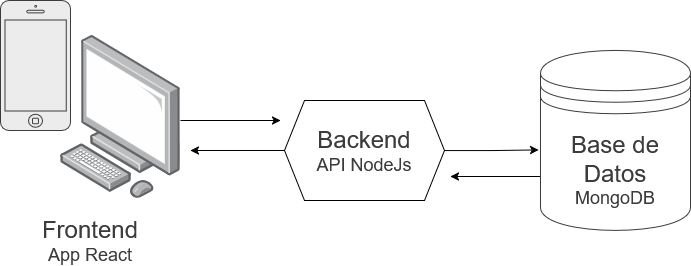
\includegraphics[width=0.9\textwidth]{./imagenes/fullstack.drawio.png}
    \caption{Arquitectura full-stack}
    \label{fig:fullstack}
\end{figure}

Al estructurar el backend exclusivamente como una API, se garantiza que el frontend sea una entidad independiente que consume recursos de forma asíncrona, optimizando la carga y mejorando la experiencia de usuario. Al decir que es una entidad independiente, se estrapola que esta API podría ser utilizada por otras aplicaciones que se construyan a futuro y quieran acceder a los servicios que la API ofrece. Esta es razón de más para testear los métodos de la API mediante la herramienta de pruebas Postman en lugar de solamente desde el frontend, dado que ayudará a comprobar y asegurar el correcto funcionamiento de éstos de forma individual, precisa y documentada.

Además, para llevar a cabo esa tarea de optimización del frontend, se ha relegado el máximo de tareas lógicas y computacionales posibles al backend. Por ejemplo, si la aplicación de React precisa de un conjunto de datos paginados, es la API la que se encargará de la paginación de estos datos, es decir, de servir estos datos por páginas mediante métodos más precisos en lugar de entregar todos los datos de golpe y dejar que el frontend los pagine, puesto que esto lo ralentizaría.

Esta sección analiza el diseño de este ecosistema, detallándolo en estas cuatro secciones:

\begin{itemize}
    \item \textbf{Stack seleccionado}: Justificación del conjunto de tecnologías escogido para el desarrollo de este proyecto de software.
    \item \textbf{Modelado de Datos NoSQL}: El uso de MongoDB y Mongoose para estructurar la información de forma flexible mediante documentos JSON modelados, facilitando el almacenamiento de estructuras de datos.

    \item \textbf{Arquitectura del backend (API REST)}: Se explica la estructura del backend, así como puntos técnicos destacados como la automatización de envío de emails, el mecanismo de autenticación, el almacenamiento de imágenes, y varias técnicas de optimización que se han implementado; y el diseño de los \textit{endpoints} (cada una de las ubicaciones donde la API recibe llamadas) y controladores que implementan las operaciones para gestionar de los datos.

    \item \textbf{Arquitectura del frontend (SPA)}: Recoge el listado de tecnologías específicas empleadas para el frontend de la aplicación, la arquitectura del proyecto, las páginas de la interfaz y, de nuevo, las técnicas de optimización aplicadas.
\end{itemize}

\section{Stack tecnológico seleccionado}

El stack tecnológico es el conjunto de herramientas, programas, aplicaciones u otras piezas de software que son utilizadas para la creación de un producto tecnológico. Una vez estudiadas las principales opciones para el desempeño de cada sector del proyecto, se cuenta con una visión global lo suficientemente rica como para hacer una elección que se ajuste a las necesidades y preferencias del proyecto y su desarrollador.

En esta sección se expone cada punto de esta selección:

\begin{itemize}
    \item Para el desarrollo del frontend de esta aplicación se ha optado por \textbf{Next.js} debido a sus ventajas en rendimiento, optimización para SEO y compatibilidad con React, que es una de las tecnologías más populares e innovadoras hoy en día, por lo que dominarlo resulta de gran interés. Entre los aspectos más atractivos de esta opción se encuentra también que cuenta con una plataforma de lanzamiento y hosting de aplicaciones gratuito, rápido y simple: Vercel; además de que la configuración inicial de un proyecto web se hace muy sencilla y existe una documentación rica, una comunidad activa y numerosos recursos para facilitar el desarrollo web.
    \item En el backend, se ha elegido \textbf{Node.js con Express} por su flexibilidad y el beneficio de utilizar el mismo lenguaje de programación, JavaScript, en todo el stack de desarrollo. Además, se trata de una tecnología ampliamente utilizada en el desarrollo de microservicios y cuenta con librerías que facilitan el acceso al tipo de base de datos que se utilizará.
    \item En cuanto a la base de datos, se ha decidido emplear \textbf{MongoDB} por su modelo flexible y su capacidad para manejar estructuras de datos dinámicas y en formato JSON, el mismo en que se manejan las estructuras de información en JavaScript. También, al ser las bases de datos relacionales las más trabajadas durante el grado, resulta de especial interés cultivar nuevas habilidades con modelos no relacionales como el de MongoDB.
    \item Para el consumo de APIs se usará \textbf{Axios} frente a FetchAPI por simplicidad y aceleración del desarrollo, dado que Axios ofrece más funcionalidades listas para usar como la conversión automática a formato JSON, el manejo de tokens o el manejo de errores integrado; mientras que Fetch, aunque es más ligero, requiere más código manual para tareas frecuentes. Dado que en esta aplicación se implementará autentifación de usuarios y una cantidad considerable de funciones, Axios se presenta como la opción más cómoda y compatible con el resto del stack.
    \item Como herramienta de pruebas de la API, se utiliza \textbf{Postman} frente a Insomnia por una razón principal: la comodidad de tenerlo ya instalado y estar familiarizada, al estar trabajando con ello en otros proyectos personales.
\end{itemize}
\begin{comment}
    \item Las inteligencias artificiles generativas que se han empleado durante la construcción del proyecto son ChatGPT para temas de investigación y clarificación de documentación, y el chat integrado de Github Copilot en Visual Studio Code por la comodidad que ofrece al trabajar directamente sobre el contexto completo del código, haciendo más eficiente y completo tanto el debugging como la entrega de propuestas de optimización y otras mejoras de los componentes y páginas.
    Por el momento, no se ha escogido ninguna plataforma de computación en la nube porque el alcance del proyecto no requiere todavía un despliegue en producción que incluya el uso de servicios externos.
\end{comment}


\subsubsection{Calidad del Código}
Adicionalmente, tanto en el frontend como en el backend, se han empleado varias herramientas destinadas a asegurar la calidad del código:

\begin{itemize}
    \item ESLint: herramienta de análisis estático configurada con reglas para mantener consistencia de código, es decir, un estilo limpio y homogéneo entre los distintos componentes, páginas y otros archivos auxiliares. También ayuda a detectar posibles errores en el código, como variables o importaciones no utilizadas.\cite{eslint_docs}
    \item TypeScript: proporciona verificación de tipos de datos en tiempo de compilación, lo cual permite detectar incompatibilidades en las propiedades de los componentes, llamadas a funciones mal tipadas, o en ocasiones el uso incorrecto de estados.
    \item Prettier: se trata de un formateador automático de código que garazantiza una aparencia consistende de este. Se han configurado reglas para limitar la longitud de línea (\texttt{printWidth: 80}), definir una indentación consistente (\texttt{tabWidth: 2}), forzar el punto y coma al final de las sentencias (\texttt{semi: true}), y estandarizar el uso de comillas dobles (\texttt{singleQuote: false}), entre otras.\cite{prettier_docs}
\end{itemize}
\section{Modelado de datos}

Para la persistencia de la información se ha optado por MongoDB, una base de datos NoSQL orientada a documentos que aporta gran flexibilidad para evolucionar el esquema ágilmente. Aunque no es estrictamente necesario al usar MongoDB, se ha optado por utilizar la librería Mongoose como ODM para definir esquemas, tipos de datos y reglas de validación para facilitar el manejo de los datos y garantizar la integridad de estos.

Así, se han estructurado los datos en diferentes colecciones, cada una de las cuales guarda registros con varios campos de diferentes tipos de datos. El modelado de datos sigue el siguiente esquema.

\begin{figure}[H]
\centering
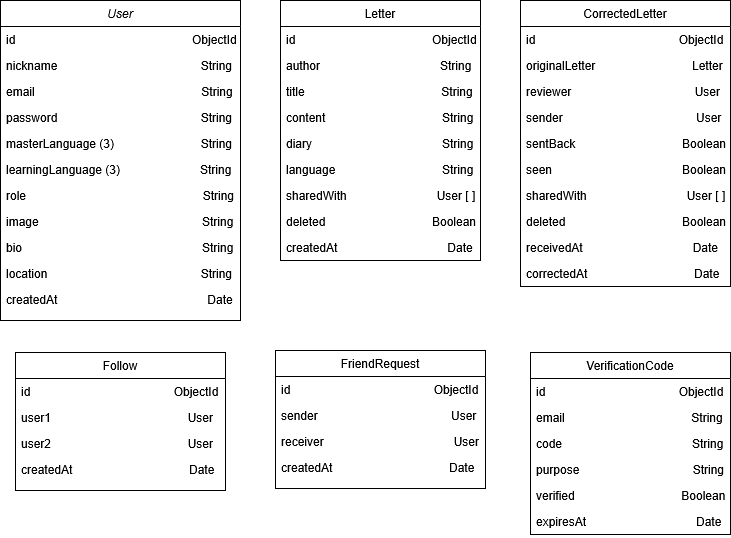
\includegraphics[width=0.8\textwidth]{./imagenes/letterexDB.png}
\caption{Estructura de Datos}
\label{fig:letterexDB}
\end{figure}

En el diseño destaca el uso del ObjectId, un identificador hexadecimal de 12 bytes que garantiza unicidad y permite la indexación eficiente basada en \textit{timestamps}. Además, facilita la vinculación mediante referencias entre colecciones. Cabe mencionar que, aunque internamente se usa \texttt{\_id}, el backend lo transforma en \texttt{id} antes de enviarlo al frontend para ofrecer una interfaz más limpia y desacoplada.

A continuación, se describen las colecciones del sistema:

\begin{itemize}
\item \textbf{Usuario (User):} gestiona la identidad y el perfil del usuario. Incluye su nombre de usuario, email, rol, imagen de perfil, biografía, localidad, contraseña, los idiomas que aprende y conoce (limitados a tres entradas por optimización técnica) y la fecha de creación.
Por seguridad, no se almacena el texto plano de la contraseña, sino que se utiliza la librería \textbf{bcrypt} con un factor de coste (\textit{salting}) de 10 para cifrar la clave antes de su persistencia. El salting es un parámetro que determina la complejidad computacional del hash para dificultar ataques de fuerza bruta al aumentar el tiempo de procesamiento necesario. Se ha escogido 10 por ser el estándar actual en la industria, aquel que se considera el punto de equilibrio óptimo entre seguridad y rendimiento. Cada vez que se quiera comprobar la contraseña, se hashea la entrada con el mismo salting y se compara el resultado con el valor guardado en la base de datos, de forma que ni el administrador ni un atacante pueda tener acceso a la contraseña.

\item \textbf{Carta (Letter):} almacena los textos originales. Contiene el author (referencia al usuario creador), título, contenido, diario, idioma y fecha de creación. También incluye un array de referencias a los usuarios con que se comparte la carta (\textit{sharedWith}) y un campo \textit{deleted} para el borrado lógico, permitiendo que los receptores conserven sus correcciones.

\item \textbf{Carta Corregida (CorrectedLetter):} gestiona el flujo de revisión. Vincula la corrección a la carta original mediante le referencia \textit{originalLetter}, además de referenciar al revisor o receptor de la carta (\textit{reviewer}) y a su autor (\textit{sender}). Controla los estados de envío de vuelta mediante el booleano \textit{sentBack}, y de si el receptor vio ya la nueva carta que le llegó con el booleano \textit{seen}, de forma que en el frontend se puedan crear etiquetas de "Nuevo" a modo de notificación. También, guarda la fecha de envío y de corrección (envío de vuelta) de la carta.

\item \textbf{Amistad (Follow):} gestiona el grafo social mediante referencias a \textit{user1} (seguidor) y \textit{user2} (seguido), facilitando el intercambio de correcciones y el listado de amigos y usuarios sugeridos.

\item \textbf{Solicitud de Amistad (FriendRequest):} capa intermedia para peticiones de amistad entre un usuario \textit{sender} y un usuario \textit{receiver}. Es una colección efímera: al aceptar o rechazar, el documento se elimina, creando el vínculo en la colección \textit{Follow} en caso de aceptación.

\item \textbf{Código de Verificación (VerificationCode):} entidad de apoyo para la validación de registros y recuperación de claves. Almacena el código hasheado, el email del usuario implicado, un campo \textit{verified} que indica si ya ha sido utilizado, y un campo \textit{purpose} que indica si sirve para un registro o para una recuperación de contraseña. Además, se utiliza un índice TTL (Time To Live) en el campo \textit{expiresAt}, que sirve para que MongoDB elimine automáticamente los códigos al cabo de 7 minutos de su creación.

\end{itemize}
\section{Arquitectura del backend}

En esta sección se expone cómo está estructurado el servidor del proyecto, los flujos lógicos que sigue, varios puntos interesantes sobre su funcionamiento, y las diferentes rutas con las que cuenta la API.

\subsection{Estructura del backend}
El servidor se organiza en módulos interconectados para ofrecer servicios robustos al frontend y facilitar un desarrollo escalable.
Una petición HTTP sigue esta secuencia: el cliente consume una ruta (endpoint), se ejecutan los middlewares de autenticación y/o carga de imágenes si corresponde, y un controlador procesa los datos interactuando con uno o varios modelos para luego devolver la respuesta que corresponda. Por ello, se distinguen los siguientes modulos principales:

\begin{itemize}
    \item \textbf{Entrada y Configuración Inicial}: En la raíz del proyecto se encuentra el archivo \texttt{index.js}, encargado de configurar y levantar el servidor. Para ello, se conecta a la base de datos y carga los endpoints y los middlewares pertinentes.

    Para que el frontend tenga acceso a la API, es esencial configurar el mecanismo de seguridad \textbf{CORS (Cross-Origin Resource Sharing)}. En una arquitectura desacoplada como la de este proyecto, el cliente y el servidor suelen operar en dominios o puertos distintos. Por seguridad, los navegadores modernos aplican la "Política de Mismo Origen" (\textit{Same-Origin Policy}), que prohíbe que un script cargado en un origen acceda a recursos de otro distinto. Con la configuración de \texttt{CORS} se define una lista de dominios autorizados a acceder a la API, así como habilitar el intercambio de credenciales.

    \begin{figure}[h]
    \centering
    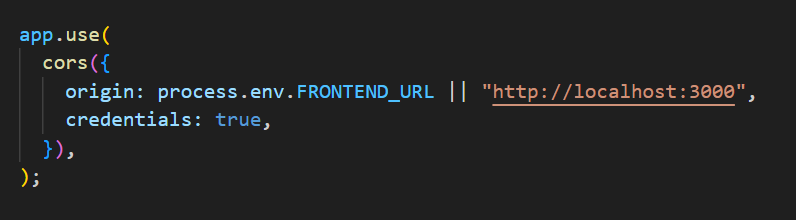
\includegraphics[width=0.8\textwidth]{imagenes/cors.png}
    \caption{Configuración del CORS en la entrada del backend}
    \label{fig:cors}
    \end{figure}

    \item \textbf{Lógica de negocio}: la lógica de negocio se organiza en una estructura con tres partes, basándose en el principio de separación por responsabilidades ("SoC" o Separation of Concerns), que busca dividir sistemas complejos en partes más pequeñas y manejables cada una de las cuales cubre una funcionalidad. Así, tenemos la definición de los puntos de acceso (\texttt{routes/}), la implementación de las reglas de negocio (\texttt{controllers/}) y la definición de los modelos de datos (\texttt{models/}).

    \item \textbf{Middlewares}: La carpeta (\texttt{middlewares/}) incluye las configuraciones de autenticación de usuario y de subida de archivos, que se explicarán en detalle más adelante.
\end{itemize}

Además, el proyecto cuenta con la carpeta \texttt{templates/}, que contiene la plantilla para enviar correos automatizados; y la carpeta \texttt{uploads/profile\_pictures/}, que actúa como almacenamiento local para las imágenes de perfil de los usuarios.


Esta separación garantiza que el sistema sea escalable y fácil de mantener.


\subsection{Emails automatizados}
La función del backend encargada la generación de códigos de verificación y su envío via email al usuario, que se emplea tanto para el registro de una nueva cuenta como para la recuperación de sus credenciales en caso de olvido; es capaz de realizar sus tareas de forma automatizada gracias a un transportador que utiliza el servicio SMTP (Simple Mail Transfer Protocol, un protocolo de red para intercambiar mensajes de correo electrónico) de Gmail. Un transportador es un objeto de configuración donde se define este servicio SMTP y se inyectan las credenciales para utilizarlo, es decir, la cuenta de correo electrónico y su contraseña.

En realidad, ya no se utiliza la contraseña de la cuenta de correo directamente, Google bloqueó eso por ser una práctica poco segura y la sustituyó por Google App Password, códigos de 16 caracteres que se pueden obtener en la configuración de la cuenta de Google y que actúan como las credenciales para usar nuestra cuenta de correo de Gmail mediante código. Estas credenciales se pueden obtener solamente al tener la 2FA (2 Factor Authentication) de Google activada, y se pueden revocar de una aplicación u otra cuando se necesite; manteniendo así las credenciales primarias seguras.

Lo que se envía en estos correos automatizados es una plantilla HTML con el código de verificación generado. De esta forma, el email que reciben los usuarios es visualmente agradable y fácil de entender en un vistazo. Así es como se ve:

\begin{figure}[H]
    \centering
    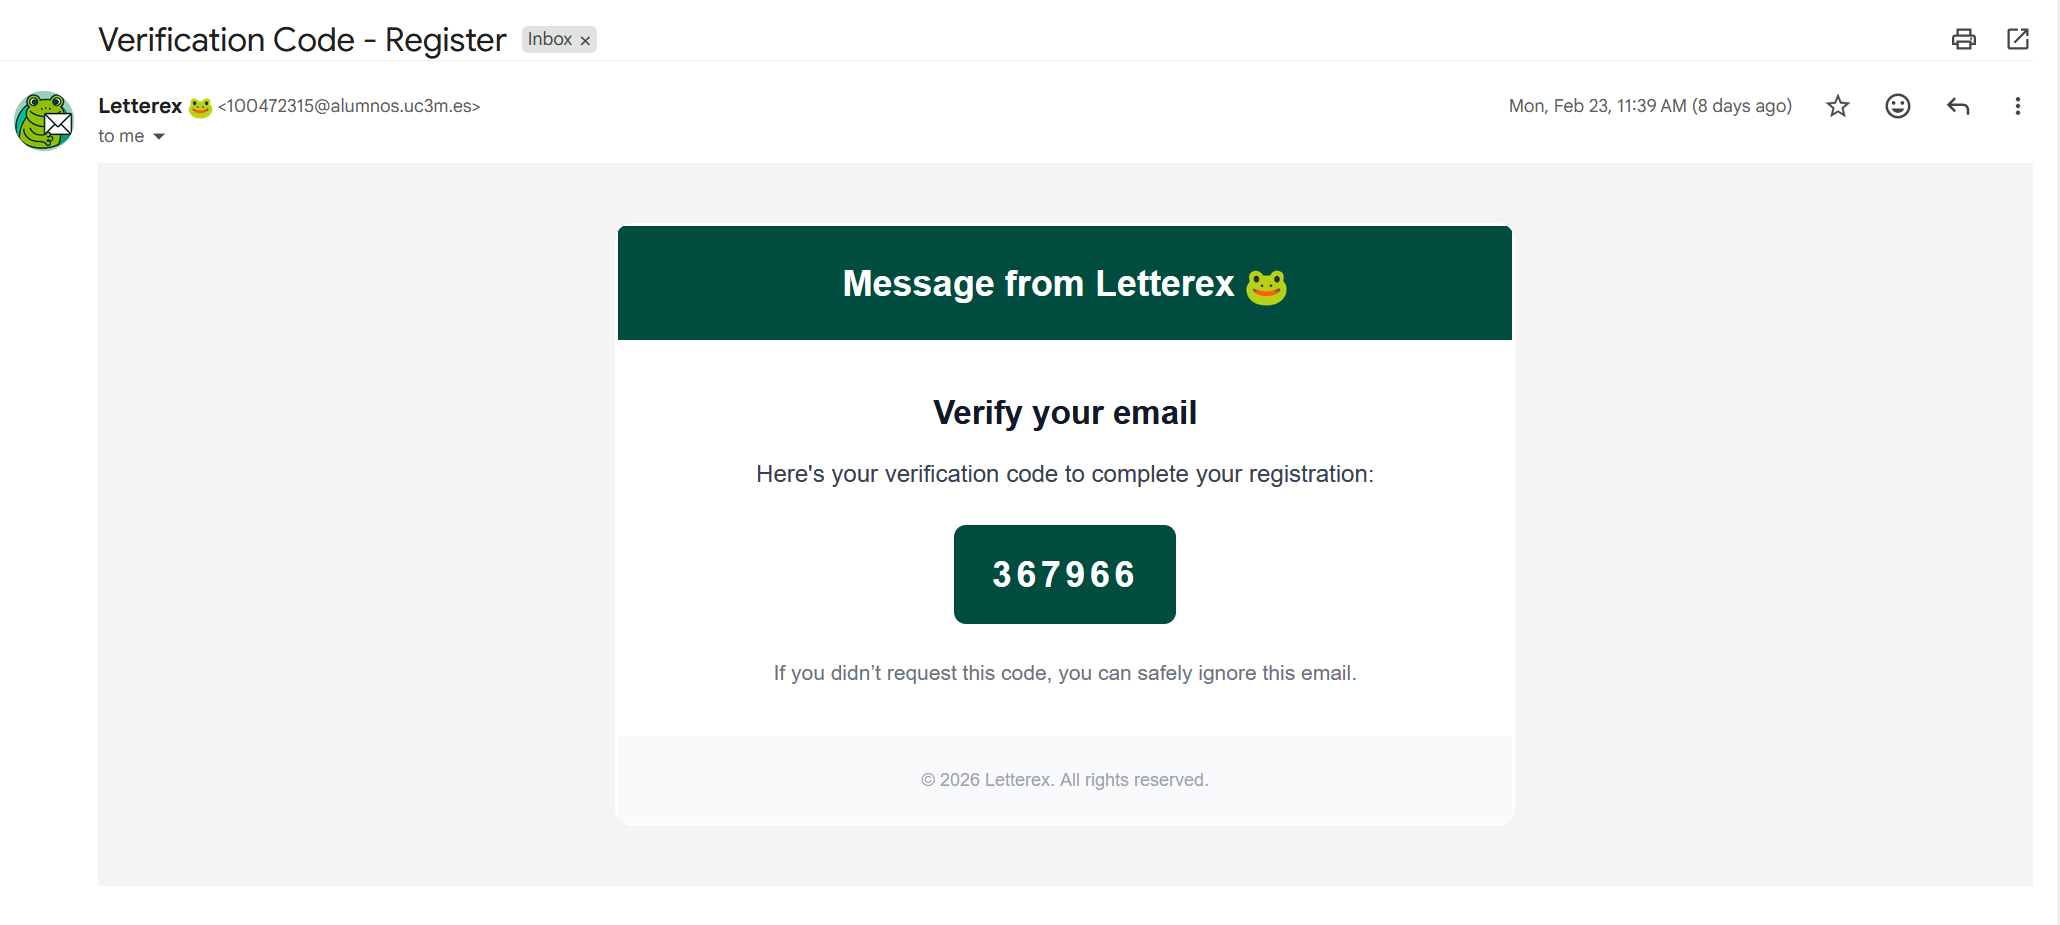
\includegraphics[width=\textwidth]{./imagenes/template_email.png}
    \caption{Email automatizado}
    \label{fig:email}
\end{figure}

\subsection{Mecanismo de Autenticación y Autorización}
Al acceder a la plataforma introduciendo su nombre de usuario o email y contraseña, el usuario recibe un token que contiene información de la sesión como el momento en que inició, el momento de caducidad, y los datos no sensibles del usuario. Se trata de un token JWT (JSON Web Token) \cite{jwtio}, un contenedor de información seguro y compacto que permite verificar la identidad del cliente en cada interacción con la API.

\begin{figure}[H]
    \centering
    
\includegraphics[height=3cm]{./imagenes/jwt.png}
    \caption{JSON Web Tokens}
    \label{fig:jwt}
\end{figure}

Este token se envia desde el backend y se almacena en el navegador mediante \textit{cookies}, con el objetivo de que el navegador pueda recordar la sesión del usuario. Al cerrar la sesión, esta cookie se elimina. El navegador adjunta automáticamente el token a las solicitudes HTTP que envía al servidor. De esta forma, el servidor es capaz de identificar al usuario y aplicar los permisos correspondientes sin necesidad de consultar una tabla de sesiones activa en la base de datos, lo que optimiza los recursos del sistema.

Sobre el refuerzo de la seguridad de la cookie, hay dos puntos interesantes que mencionar. En primer lugar, la cookie es HttpOnly, es decir, no se puede leer mediante JavaScript sino que solo puede leerla el navegador. De esta forma, el token está protegido contra ataques maliciosos como \textbf{Cross-Site Scripting (XSS)}, una vulnerabilidad en la que un atacante inyecta y ejecuta código malicioso (generalmente de JavaScript) en el navegador de otros usuarios que usan la aplicación.

En segundo lugar, se ha implementado el atributo \textbf{SameSite} con el valor \texttt{"Strict"}. Esta configuración es una medida de seguridad crítica para prevenir ataques de tipo \textbf{CSRF (Cross-Site Request Forgery)}, que aprovechan la naturaleza automática de los navegadores, dado que estos adjuntan las cookies de sesión a cualquier petición dirigida al dominio de origen. El atacante podría engañar a un usuario autenticado para que haga clic en un enlace malicioso en una pestaña diferente, y dicho enlace dispararía una petición a nuestra API (por ejemplo, para borrar una carta o cambiar la contraseña). Con la configuración de SameSite, este tipo de ataques son mitigados.

Al llegar una solicitud HTTP al sistema, si se trata de una ruta protegida se ejecuta el \textbf{Middleware de Autenticación}. Este componente intercepta la solicitud, extrae el token JWT de la cookie y verifica su validez. Si es válido, el middleware decodifica la información del usuario y la inyecta en el objeto de la petición, permitiendo que el resto del flujo identifique al autor de la acción, es decir, el usuario autenticado en la aplicación.

Estas decisiones técnicas refuerzan la robustez del sistema y aseguran que cada acción realizada en este sea legítima y provenga exclusivamente de la interacción directa del usuario con la interfaz oficial, de forma que usuario pueda acceder de forma segura a las acciones que requieren su autenticación.

\subsection{Almacenamiento de imágenes con Multer y Cloudinary}

Para la gestión de imágenes de perfil, se ha implementado una solución que combina la librería \textbf{Multer} para el procesamiento eficiente de archivos con \textbf{Cloudinary} como servicio de almacenamiento en la nube. Multer es una librería que facilita la subida de archivos mediante formularios web para aplicaciones de Node.js. Por su parte, Cloudinary es un servicio de gestión de recursos digitales, en especial imágenes y vídeos, que proporciona almacenamiento persistente en la nube y optimización automática. \cite{llamas_multer_nd, cloudinary_official_2026,moge_cloudinary_2026}

La configuración del sistema de subida de archivos se divide en tres pilares fundamentales:

\begin{itemize}
    \item Procesamiento en memoria: Se utiliza Multer para interceptar y procesar la subida de archivos directamente en memoria con un búfer, evitando la necesidad de almacenamiento temporal en disco. Una decisión de diseño clave ha sido el renombrado del archivo por el identificador del usuario extraído del token de autenticación, de modo que cada usuario posea una única imagen de perfil en Cloudinary. En caso de actualización, se sobrescribe la imagen anterior automáticamente, eliminando la necesidad de gestionar manualmente archivos obsoletos.

    \item Almacenamiento en la nube: Una vez procesado el búfer, la imagen se sube directamente a Cloudinary. El sistema almacena la URL segura retornada por Cloudinary en la base de datos, facilitando un acceso rápido sin depender del almacenamiento local del servidor. Además, Cloudinary aplica transformaciones automáticas, como la limitación de dimensiones a 800x800 píxeles, para garantizar consistencia visual y reducir consumo de ancho de banda.
    \item Filtrado de seguridad: Para prevenir la subida de archivos maliciosos (como \textit{scripts} ejecutables disfrazados), se ha implementado un filtro por tipo MIME y extensión. El sistema solo acepta formatos de imagen estándar (\texttt{JPEG, JPG, PNG}), verificando tanto la extensión del archivo como su tipo MIME real para asegurar la integridad del recurso. También, se establece un máximo de tamaño del archivo de 5 MB para evitar \textbf{ataques de denegación de servicio (DoS)} por agotamiento de almacenamiento o ancho de banda.

\end{itemize}

Este módulo se exporta como un middleware independiente, lo que permite inyectarlo exclusivamente en las rutas de la API que requieren capacidad de subida, manteniendo así el principio de responsabilidad única en el código. Además, la integración con Cloudinary elimina la dependencia de la infraestructura local de almacenamiento, proporcionando escalabilidad y disponibilidad.

\subsection{Interfaz de Programación de Aplicaciones (API): Rutas y Controladores}

El backend de la plataforma actúa como una capa de servicios diseñada para que el frontend interactúe con la base de datos de forma segura y eficiente. Esta comunicación se articula mediante una \textbf{API RESTful}, que expone una serie de puntos de entrada o endpoints organizados por recursos (usuarios, cartas, correcciones, etc.).

La lógica de interacción se fundamenta en las operaciones \textbf{CRUD} (\textit{Create, Read, Update, Delete}), que representan las acciones esenciales para la gestión de persistencia de datos. En este proyecto, dichas acciones se mapean directamente con los métodos del protocolo \textbf{HTTP}, garantizando una arquitectura estandarizada:

\begin{itemize}
    \item \textbf{POST (Create)}: Utilizado para la creación de nuevos documentos, como el registro de un usuario o el envío de una nueva carta.
    \item \textbf{GET (Read)}: Empleado para la recuperación de información, ya sea una lista de recursos o un documento específico identificado por su ID.
    \item \textbf{PUT / PATCH (Update)}: Destinados a la actualización de registros existentes. Se utiliza \texttt{PUT} para sustituciones integrales y \texttt{PATCH} para modificaciones parciales, como marcar una carta como "leída".
    \item \textbf{DELETE (Delete)}: Encargado de la eliminación de recursos o, en el caso de las cartas, de la activación del borrado lógico mencionado anteriormente.
\end{itemize}

Cada ruta definida en el servidor está vinculada a un \textbf{controlador} específico, el cual contiene la lógica final para procesar la solicitud. Una vez superada la fase de autenticación, la ejecución pasa al controlador específico correspondiente, cuya función es extraer los parámetros de la consulta, utilizar la identidad del usuario ya validada para aplicar reglas de negocio, ejecutar las operaciones correspondientes en MongoDB mediante los modelos de Mongoose, y devolver una respuesta HTTP con los datos en formato JSON y un código de éxito o error.

A continuación, se muestra una tabla con todos los métodos que se han desarrollado para esta API y de los que el frontend más adelante se servirá. Estás separados en categorías según el controlador y enrutador que se encarga de ellos: User, Letter, CorrectedLetter y Follow. Podría crearse uno nuevo para los modelos de VerificationCode y FriendRequest, pero por simplicidad se han incluido las pocas funciones de estos en el grupo de User y Follow, respectivamente. Además, se marca con un asterisco los valores de entrada obligatorios.

\begin{longtable}{|l|p{5cm}|p{8cm}|}
\hline
\textbf{Función} & \textbf{Ruta} & \textbf{Descripción} \\
\hline
\endhead
\hline
\endfoot
\multicolumn{3}{|c|}{\textbf{User Routes}} \\
\hline
POST & /api/users/register & Registrar un nuevo usuario. \newline \textbf{Valores de entrada:} nickname*, email*, password*, master\-Language*, learning\-Language* \newline \textbf{Valores de salida:} status, message, user \\
POST & /api/users/login & Iniciar sesión. Si las credenciales recibidas son correctas, se crea y envía la cookie de autenticación. \newline \textbf{Valores de entrada:} email* (string, puede ser email o nickname), password* \newline \textbf{Valores de salida:} status, userData, token, cookie authToken \\
POST & /api/users/logout & Cerrar la sesión. Se limpia la cookie de autenticación. \newline \textbf{Valores de entrada:} ninguno \newline \textbf{Valores de salida:} status, message \\
GET & /api/users/profile/:id? & Obtener los datos del perfil de usuario cuyo id es especificado en la ruta, o en su defecto (es un parámetro opcional, de ahí el signo de interrogación en la ruta) del usuario autenticado.\newline \textbf{Valores de salida:} status, user \\
GET & /api/users/list-users/:page? & Listar usuarios con paginación. Si no se recibe el parámetro page, que indica la página que se pide, se entregan los usuarios de la primera página. \newline \textbf{Valores de salida:} status, users, page, itemsPerPage, totalUsers, totalPages \\
PUT & /api/users/update & Actualizar datos del usuario autenticado. \newline \textbf{Valores de salida:} status, userData \\
PUT & /api/users/change-password & Cambiar contraseña actual. \newline \textbf{Valores de salida:} status, message \\
PUT & /api/users/profile-picture & Subir foto de perfil. Se trata de un método PUT porque no solo sube una nueva imagen al sistema de archivos sino que modifica los datos del usuario.\newline \textbf{Valores de salida:} status, userId, profilePicture \\
DELETE & /api/users/profile-picture & Eliminar foto de perfil. \newline \textbf{Valores de salida:} status, message \\
GET & /api/users/profile-picture/:id & Obtener foto de perfil de un usuario. En caso de que el parámetetro id no esté especificado, se entrega la del usuario autenticado. \newline \textbf{Valores de salida:} Archivo (imagen) \\
GET & /api/users/check-nickname/:nickname & Verificar disponibilidad de nickname. \newline \textbf{Valores de salida:} status, inUse: boolean \\
GET & /api/users/check-email/:email & Verificar si email está registrado. \newline \textbf{Valores de salida:} result, inUse: boolean \\
POST & /api/users/verification-code & Enviar código de verificación. \newline \textbf{Valores de entrada:} email*, purpose \newline \textbf{Valores de salida:} message \\
POST & /api/users/check-code & Verificar código de verificación. \newline \textbf{Valores de entrada:} email*, code*, purpose \newline \textbf{Valores de salida:} status, message \\
PUT & /api/users/reset-password & Restablecer contraseña con código de verificación. \newline \textbf{Valores de salida:} status, message \\
DELETE & /api/users/delete-account & Eliminar cuenta de usuario. \newline \textbf{Valores de salida:} status, message \\
\hline
\hline
\multicolumn{3}{|c|}{\textbf{Letter Routes}} \\
\hline
POST & /api/letters/new & Guardar una carta nueva. \newline \textbf{Valores de entrada:} title*, content*, language*, created\_at*, diary \newline \textbf{Valores de salida:} status, message, letter \\
GET & /api/letters/view/:letterId & Obtener información y contenido de una carta.\newline \textbf{Valores de salida:} status, letter, sharedWithDetails \\
PUT & /api/letters/edit/:id & Editar una carta existente. \newline \textbf{Valores de salida:} status, message, letter \\
PUT & /api/letters/edit-diary & Editar el diario de una carta. \newline \textbf{Valores de salida:} status, message, letter \\
DELETE & /api/letters/delete/ & Eliminar una o varias cartas. \newline \textbf{Valores de salida:} status, message \\
GET & /api/letters/list & Listar todas las cartas del usuario. \newline \textbf{Valores de salida:} status, letters, count \\
GET & /api/letters/list/search & Buscar cartas por título. \newline \textbf{Valores de salida:} status, letters \\
POST & /api/letters/share/:id & Compartir una carta con otro usuario (uno o varios). \newline \textbf{Valores de entrada:} shared\-With* \newline \textbf{Valores de salida:} \{message, letter, correctedLetters\} \\
GET & /api/letters/diaries & Listar diarios del usuario. \newline \textbf{Valores de salida:} status, diaries \\
GET & /api/letters/count/:id? & Contar cartas por idioma. Si no se especifica id en la ruta, se cuentan las del usuario autenticado. \newline \textbf{Valores de salida:} Array de \{language, count\} \\
\hline
\hline
\multicolumn{3}{|c|}{\textbf{Follow Routes}} \\
\hline
POST & /api/follow/add/:id & Mandar una solicitud de amistad a un usuario. \newline \textbf{Valores de salida:} status, message \\
DELETE & /api/follow/unfollow/:id & Dejar de seguir a un usuario. \newline \textbf{Valores de salida:} status, message \\
GET & /api/follow/request/:id & Verificar si existe solicitud de amistad. \newline \textbf{Valores de salida:} status, exists: boolean \\
GET & /api/follow/friends & Obtener lista de amigos. \newline \textbf{Valores de salida:} status, count, friends \\
GET & /api/follow/non-friends & Obtener usuarios no agregados. \newline \textbf{Valores de salida:} status, users, totalUsers, totalPages \\
GET & /api/follow/non-friends/:filter & Obtener no usuarios no agregados con un filtro por su nickname. \newline \textbf{Valores de salida:} status, users, totalUsers, totalPages \\
GET & /api/follow/suggested & Obtener usuarios sugeridos. Son usuarios a los que el usuario autenticado no sigue y que tienen idiomas en común con este. \newline \textbf{Valores de salida:} status, suggestedUsers \\
POST & /api/follow/request/:id & Enviar solicitud de amistad. \newline \textbf{Valores de salida:} status, message, friendRequest \\
GET & /api/follow/requests & Listar solicitudes de amistad recibidas. \newline \textbf{Valores de salida:} status, requests \\
POST & /api/follow/accept/:id & Aceptar solicitud de amistad. \newline \textbf{Valores de salida:} status, message \\
POST & /api/follow/decline/:id & Rechazar solicitud de amistad. \newline \textbf{Valores de salida:} status, message \\
\hline
\hline
\multicolumn{3}{|c|}{\textbf{Corrected Letter Routes}} \\
\hline
PATCH & /api/corrected-letters/send-back/:corrected\-Letter\-Id & Mandar de vuelta su autor la carta corregida. \newline \textbf{Valores de salida:} status, message, correctedLetter \\
GET & /api/corrected-letters/corrections/:original\-Letter\-Id & Obtener correcciones de una carta. \newline \textbf{Valores de salida:} status, corrections \\
GET & /api/corrected-letters/corrected\-Letter/:corrected\-Letter\-Id & Obtener corrección específica por ID. \newline \textbf{Valores de salida:} status, correctedLetter \\
GET & /api/corrected-letters/received/ & Obtener cartas recibidas para corregir. \newline \textbf{Valores de salida:} status, correctedLetters, count \\
GET & /api/corrected-letters/received/search & Buscar cartas recibidas por un filtro "search". \newline \textbf{Valores de salida:} status, correctedLetters \\
PUT & /api/corrected-letters/update/:corrected\-Letter\-Id & Actualizar correcciones en proceso. Si la carta ya ha sido enviada de vuelta no se puede realizar esta acción. \newline \textbf{Valores de salida:} status, message, correctedLetter \\
GET & /api/corrected-letters/count/:id? & Contar cartas corregidas por idioma. Si no se especifica el id de usuario en la ruta, se cuentan las del usuario autenticado. \newline \textbf{Valores de salida:} Array de \{language, count\} \\
DELETE & /api/corrected-letters/:corrected\-Letter\-Id & Eliminar carta corregida. \newline \textbf{Valores de salida:} status, message \\
\hline
\caption{Rutas de la API de Letterex}
\label{tab:rutas-api}
\end{longtable}



\subsection{Técnicas de optimización}

\subsubsection{Optimización de búsqueda datos}
La lógica de filtrado se procesa íntegramente en el servidor para garantizar la escalabilidad y mejorar la velocidad de la interfaz liberándola de tareas programacionales. El controlador recibe los términos de búsqueda y ejecuta una consulta optimizada en MongoDB. Esto reduce drásticamente el tamaño de los datos transferidos a través de la red en comparación con un filtrado realizado en el lado del cliente sobre la totalidad de los registros.

Además, para mejorar la usabilidad en la búsqueda y filtrado de cartas, se ha implementado un sistema de comunicación eficiente entre el cliente y el servidor. Donde tenemos una barra de búsqueda, en lugar de realizar peticiones por cada pulsación de tecla, lo que derivaría en un consumo excesivo de recursos y latencia en la red, se ha aplicado la técnica de \textbf{debouncing}. Esta técnica sigue la siguiente lógica:

\begin{itemize}
    \item Control de Eventos: Cuando el usuario escribe en el campo de búsqueda, se inicia un temporizador interno.
    \item Retraso Controlado: Si el usuario sigue escribiendo antes de que transcurran un intervalo definido de tiempo (500ms), el temporizador se reinicia.
    \item Petición Asíncrona: Solo cuando el usuario deja de escribir durante el tiempo estipulado, se dispara la solicitud formal a la API.
\end{itemize}

Así, se logra un consumo y envío de recursos mucho más eficiente.

\subsubsection{Procesamiento Avanzado de Datos: Aggregate de MongoDB}

Otra forma de optimización clave utilizada en el desarrollo del backend es el uso del Aggregate o operaciones de agregación de MongoDB \cite{mongodb_aggregation_2026}. Esta herramienta permite acceder a diferentes colecciones y aplicar filtrados, ordenamientos, uniones, proyecciones y paginación en una única operación atómica. Esto evita el procesar grandes volúmenes de datos en la capa de JavaScript o caer en el problema de las \textbf{N+1 consultas} (realizar múltiples peticiones a la base de datos para completar un solo registro). Así, delegamos la carga de procesamiento al motor de la base de datos, manteniendo tiempos de respuesta bajos y escalables.

\begin{comment}
Un ejemplo real implementado es el flujo de trabajo para la búsqueda de cartas, donde se obtienen también los detalles de los usuarios que han enviado correcciones. El proceso se divide en las siguientes etapas:

    \item \textbf{Pre-filtrado y Paginación}: Primero se selecciona un conjunto reducido de documentos mediante un \texttt{\$match} (autor logueado y carta no eliminada), un \texttt{\$sort} cronológico y las etapas \texttt{\$skip} y \texttt{\$limit} para gestionar la paginación. Realizar esto al inicio asegura que las operaciones posteriores, más costosas, solo se apliquen a los resultados visibles.

    \item \textbf{Resolución de Identidades}: Se aplica un \texttt{\$lookup} (equivalente al \textit{join} de SQL) para unir la colección de cartas con la de usuarios. Esto permite resolver los IDs del array \texttt{sharedWith} y obtener los perfiles reales de los destinatarios.

    \item \textbf{Búsqueda de Correcciones}: Seguidamente, se realiza un segundo cruce con la colección CorrectedLetter. Para cada carta, el sistema busca documentos donde la carta original coincida con la actual y el campo \texttt{sentBack} sea verdadero, agrupando estos resultados en un array interno.

    \item \textbf{Transformación de la Salida}: Finalmente, se formatea la respuesta final procesando el array de amigos mediante el operador \texttt{\$map} de MongoDB. Este transforma cada elemento verificando si el ID del amigo existe en el array de revisores (usando \texttt{\$in}) y extrayendo el ID específico de la corrección mediante la combinación de \texttt{\$filter} y \texttt{\$arrayElemAt}.
\end{comment}

Un ejemplo representativo es el flujo de obtención de cartas junto con la información de sus correcciones y usuarios asociados. La tubería de agregación de MongoDB permite resolver estas múltiples relaciones en una única consulta. El proceso se estructura en las siguientes etapas:

\begin{enumerate}
    \item \textbf{Filtrado y paginación}: Se seleccionan únicamente las cartas del usuario autenticado que no han sido eliminadas, aplicando además ordenación cronológica y paginación. Realizar esto al inicio asegura que las operaciones posteriores, más costosas, solo se apliquen a los resultados deseados.

    \item \textbf{Enriquecimiento de datos}: Se incorporan los datos de los usuarios relacionados, aquellos con los que se ha compartido la carta, mediante operaciones equivalentes a uniones (\textit{joins}), resolviendo los identificadores almacenados en el campo \texttt{sharedWith}.

    \item \textbf{Obtención de correcciones}: Se recuperan las correcciones asociadas a cada carta, filtrando para obtener solamente aquellas que han sido enviadas de vuelta al autor.

    \item \textbf{Transformación de la respuesta}: Finalmente, se construye la estructura de salida combinando la información obtenida, de forma que cada carta incluye los datos necesarios para su representación en la interfaz.
\end{enumerate}

Aunque construir esta lógica requiere mayor tiempo de desarrollo, el uso de la Agregación de MongoDB permite una mejora drástica en el rendimiento del sistema reduciendo el tráfico de red entre el servidor y la base de datos.

A continuación se muestra el código de la función que se ha presentado como ejemplo de su uso.

\begin{figure}[H]
    \centering
    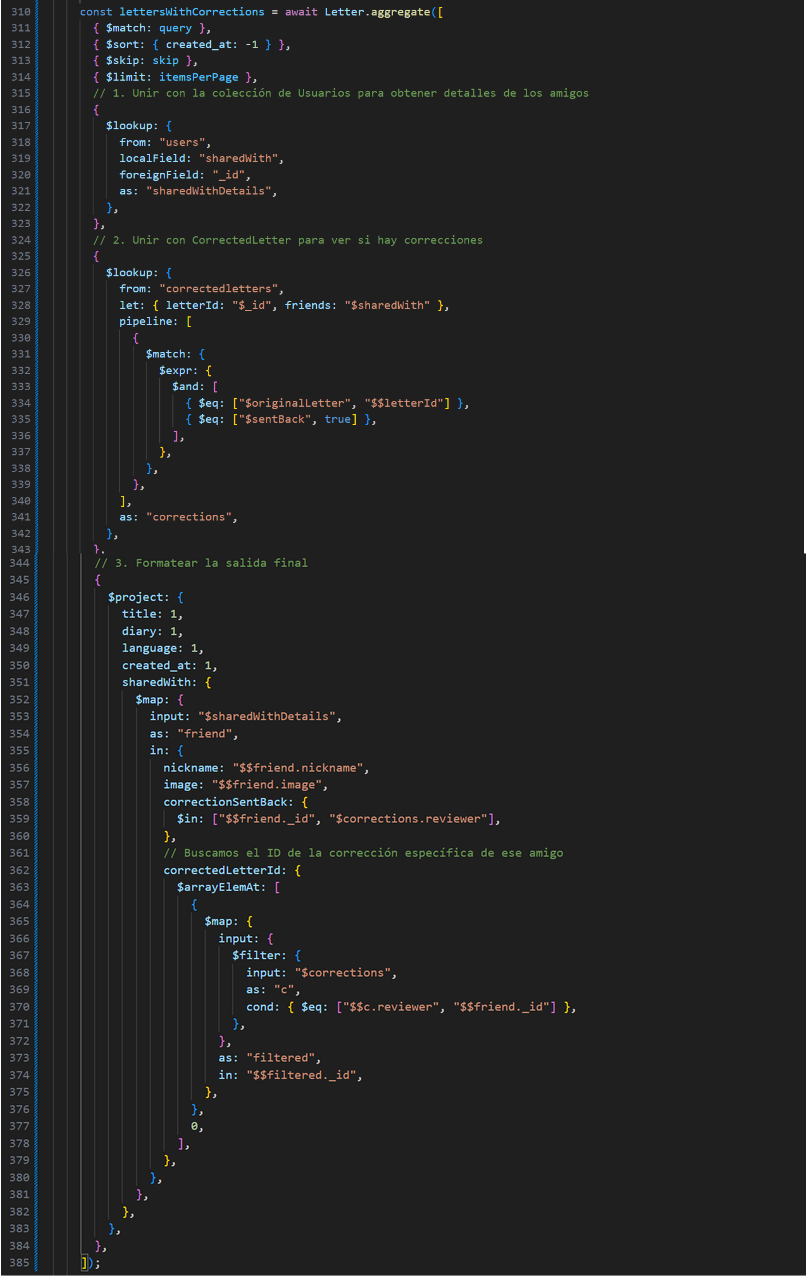
\includegraphics[width=\textwidth]{./imagenes/aggregate3.png}
    \caption{Consulta optimizada 1}
    \label{fig:aggregate}
\end{figure}
\section{Frontend de la aplicación}

El frontend ha sido desarrollado como una aplicación web moderna y responsiva, utilizando las últimas tecnologías del ecosistema React. En esta sección, se presentan las diferentes tecnologías que han intervenido en el desarrollo de esta pieza de software, la arquitectura que sigue el proyecto de frontend, las diferentes páginas que lo componen, y varias técnicas de optimización que se han empleado.


\subsection{Stack Tecnológico}

La aplicación se ha construido utilizando el siguiente stack tecnológico:

\begin{itemize}
    \item React 19: Biblioteca principal para la construcción de interfaces de usuario basadas en componentes.
    \item Next.js 15: Framework de React que proporciona renderizado del lado del servidor (SSR), enrutamiento basado en archivos y optimizaciones de rendimiento automáticas.
    \item TypeScript: Superset tipado de JavaScript que proporciona seguridad de tipos en tiempo de compilación.
    \item Tailwind CSS: Framework de CSS utility-first para un desarrollo de estilos rápido y consistente. El uso este librería agiliza la aplicación de interfaces responsivas, adaptándose a todo tipo de dispositivos con tamaños de pantalla diversos.
    \item Framer Motion: Biblioteca de animaciones para crear transiciones fluidas y experiencias interactivas.\cite{framer_motion_docs}
    \item React Quill: Editor de texto enriquecido basado en Quill.js para la escritura de cartas.\cite{quill_react_playground}
    \item Axios: Cliente HTTP para comunicación con la API backend.
    \item React Leaflet: Biblioteca para integración de mapas interactivos.\cite{react_leaflet_docs}
\end{itemize}

\subsection{Arquitectura del Frontend y Gestión del Estado}

El proyecto sigue la estructura de \textit{App Router} de Next.js 13+, que organiza las rutas de la aplicación en función de la estructura de directorios. La estructura consta de las siguientes capas:

\begin{itemize}
    \item \texttt{app/}: Directorio principal que contiene las páginas y rutas de la aplicación. Cada subcarpeta se convierte en una ruta de la web automáticamente si incluimos dentro un archivo \texttt{page.tsx}.
    \item \texttt{components/}: Componentes reutilizables de la interfaz de usuario.
    \item \texttt{services/}: Capa de servicios que encapsula las llamadas a la API.
    \item \texttt{context/}: Contextos de React para gestión de estado global.
    \item \texttt{lib/}: Utilidades, tipos de TypeScript y constantes.
    \item \texttt{stylesheets/}: Aunque los estilos se aplican mayoritariamente con Tailwind CSS, para ciertos casos se utilizan estilos personalizados complementarios compartidos por varios componentes.
\end{itemize}


Para facilitar la escalabilidad y la reutilización del código, se han desarrollado \textbf{componentes reutilizables} para encapsular elementos como botones, inputs, selectores, descripciones emergentes, etc. Estos se incluyen en diferentes páginas y componentes de la aplicación para garantizar patrones de diseño consistentes, evitar la duplicación de lógica, y facilitar la implementación de cambios globales.

En cuanto a la \textbf{comunicación con el backend}, la capa de servicios encapsula toda la lógica de acceso a la API, que se implementa con Axios. La capa incluye cuatro módulos diferenciados por funcionalidad: usuarios, cartas, correcciones y amistades. Cada módulo de servicio exporta funciones asíncronas que manejan configuración de headers de autenticación, errores HTTP y de Axios, transformación de datos entre el formato de la API y el formato esperado por los componentes; y validación básica de datos antes del envío.

Respesto a la gestión del estado de la aplicación, se deben almacenar ciertos datos comunes a todas o varias páginas, así como datos individuales de cada página o componente. Para ello, se utilizan múltiples estrategias:

\begin{itemize}
    \item \textbf{Local Storage}: Utilizado para datos no sensibles de la experiencia de usuario, como la preferencia de tema (modo claro u oscuro), que se establece inicialmente como el que tenga por defecto el usuario en su navegador, pero puede ser configurarse desde el menú desplegable de Letterex.
    \item \textbf{React Hooks}: Se usan funciones especiales de React como \texttt{useState}, \texttt{useEffect} o \texttt{useRef}, para controlar el estado local de los componentes. Este último se usa para implementar una caché en memoria por página, por ejemplo, guardando resultados paginados. Cuando el usuario vuelve a una página ya consultada, los datos se leen desde caché y se muestran al instante. Así, se consigue una mejora del rendimiento por la reducción de llamadas redundantes al servidor.
    \item \textbf{Context API}: guarda el estado del componente para gestionar diálogos modales de forma centralizada, evitando \textit{prop drilling}, fenónemo en que los componentes se pasan datos de padres a hijos sucesivamente quedando varios hijos intermedios que no los utilizan. Con un proveedor de contexto, la app es capaz de renderizar un solo componente de diálogo que se abre y se cierra con dos funciones a las que cualquier componente puede acceder fácilmente, en este caso mediante un hook personalizado llamado \texttt{useDialog} que devuelve el contexto del diálogo. Por ejemplo, la siguiente figura muestra la función que abrirá el diálogo de error a su derecha. Esta estrategia se utiliza también para guardar los datos no sensibles del usuario autenticado.

    \begin{figure}[H]
        \centering
        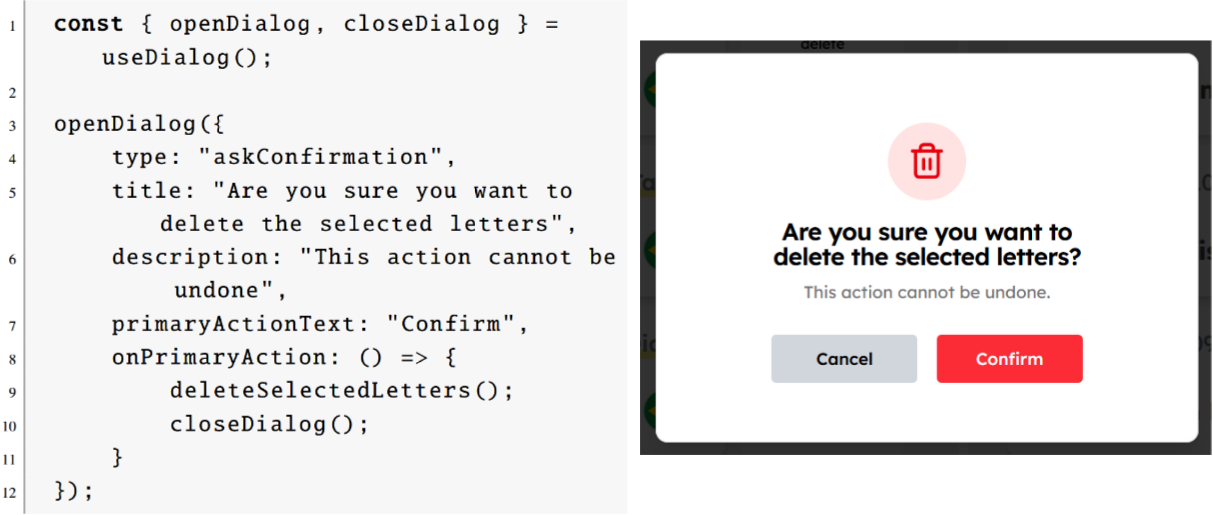
\includegraphics[width=\textwidth]{imagenes/ui/dialogDeleteAll.png}
        \caption{Código de apertura del diálogo y resultado en la interfaz}
        \label{fig:dialog}
    \end{figure}

\end{itemize}



\subsection{Páginas de la aplicación}

En este apartado se irán mostrando las diferentes páginas que componen la interfaz, que en total son siete: la página de inicio de sesión, la página principal, la página para la creación de una nueva carta, la página de correción de cartas recibidas, la página de visualización de una correción recibida, la página de amigos, y la página de perfil de usuario.

En las paginas protegidas (aquellas a las que se accede tras iniciar sesión), el componente \texttt{Sidebar} envuelve todo el contenido para proporcionar una barra lateral de navegación persistente con acceso rápido a todas las páginas de la aplicación.

\subsubsection{Página de Inicio y Autenticación}

\begin{figure}[h]
    \centering
    
\includegraphics[width=\textwidth]{imagenes/ui/login.png}
    \caption{Página de inicio de sesión y registro}
    \label{fig:landing}
\end{figure}

La página de inicio presenta una interfaz atractiva y animada que da la bienvenida a los usuarios. Esta página utiliza el componente \texttt{AnimatedForm} que gestiona tres estados principales:

\begin{itemize}
    \item \textbf{Bienvenida}: Presenta el propósito de la aplicación con un efecto de escritura animado (\textit{typewriter}) que muestra frases como ``Write about your passions'', ``Exchange language corrections'' y ``Find people to share and learn'', para dar una idea general de aquello en que consiste la plataforma.
    \item \textbf{Inicio de sesión}: Formulario de inicio de sesión para usuarios existentes.
    \item \textbf{Registro}: Formulario de registro con verificación de email mediante el código enviado a su correo, selección de idioma nativo e idiomas de interés, selección de contraseña y nombre de usuario, y posibilidad de subir una foto de perfil.
    \item \textbf{Olvido de contraseña}: Formulario que permite resetear la contraseña del usuario mediante el código de verificación enviado a su email.
\end{itemize}

Una característica distintiva de esta página es la animación del logo implementada con Framer Motion, que se desplaza suavemente entre diferentes posiciones según el formulario activo, proporcionando un elemento lúdico y memorable a la experiencia del usuario.
\subsubsection{Página Principal}

\begin{figure}[h]
    \centering
    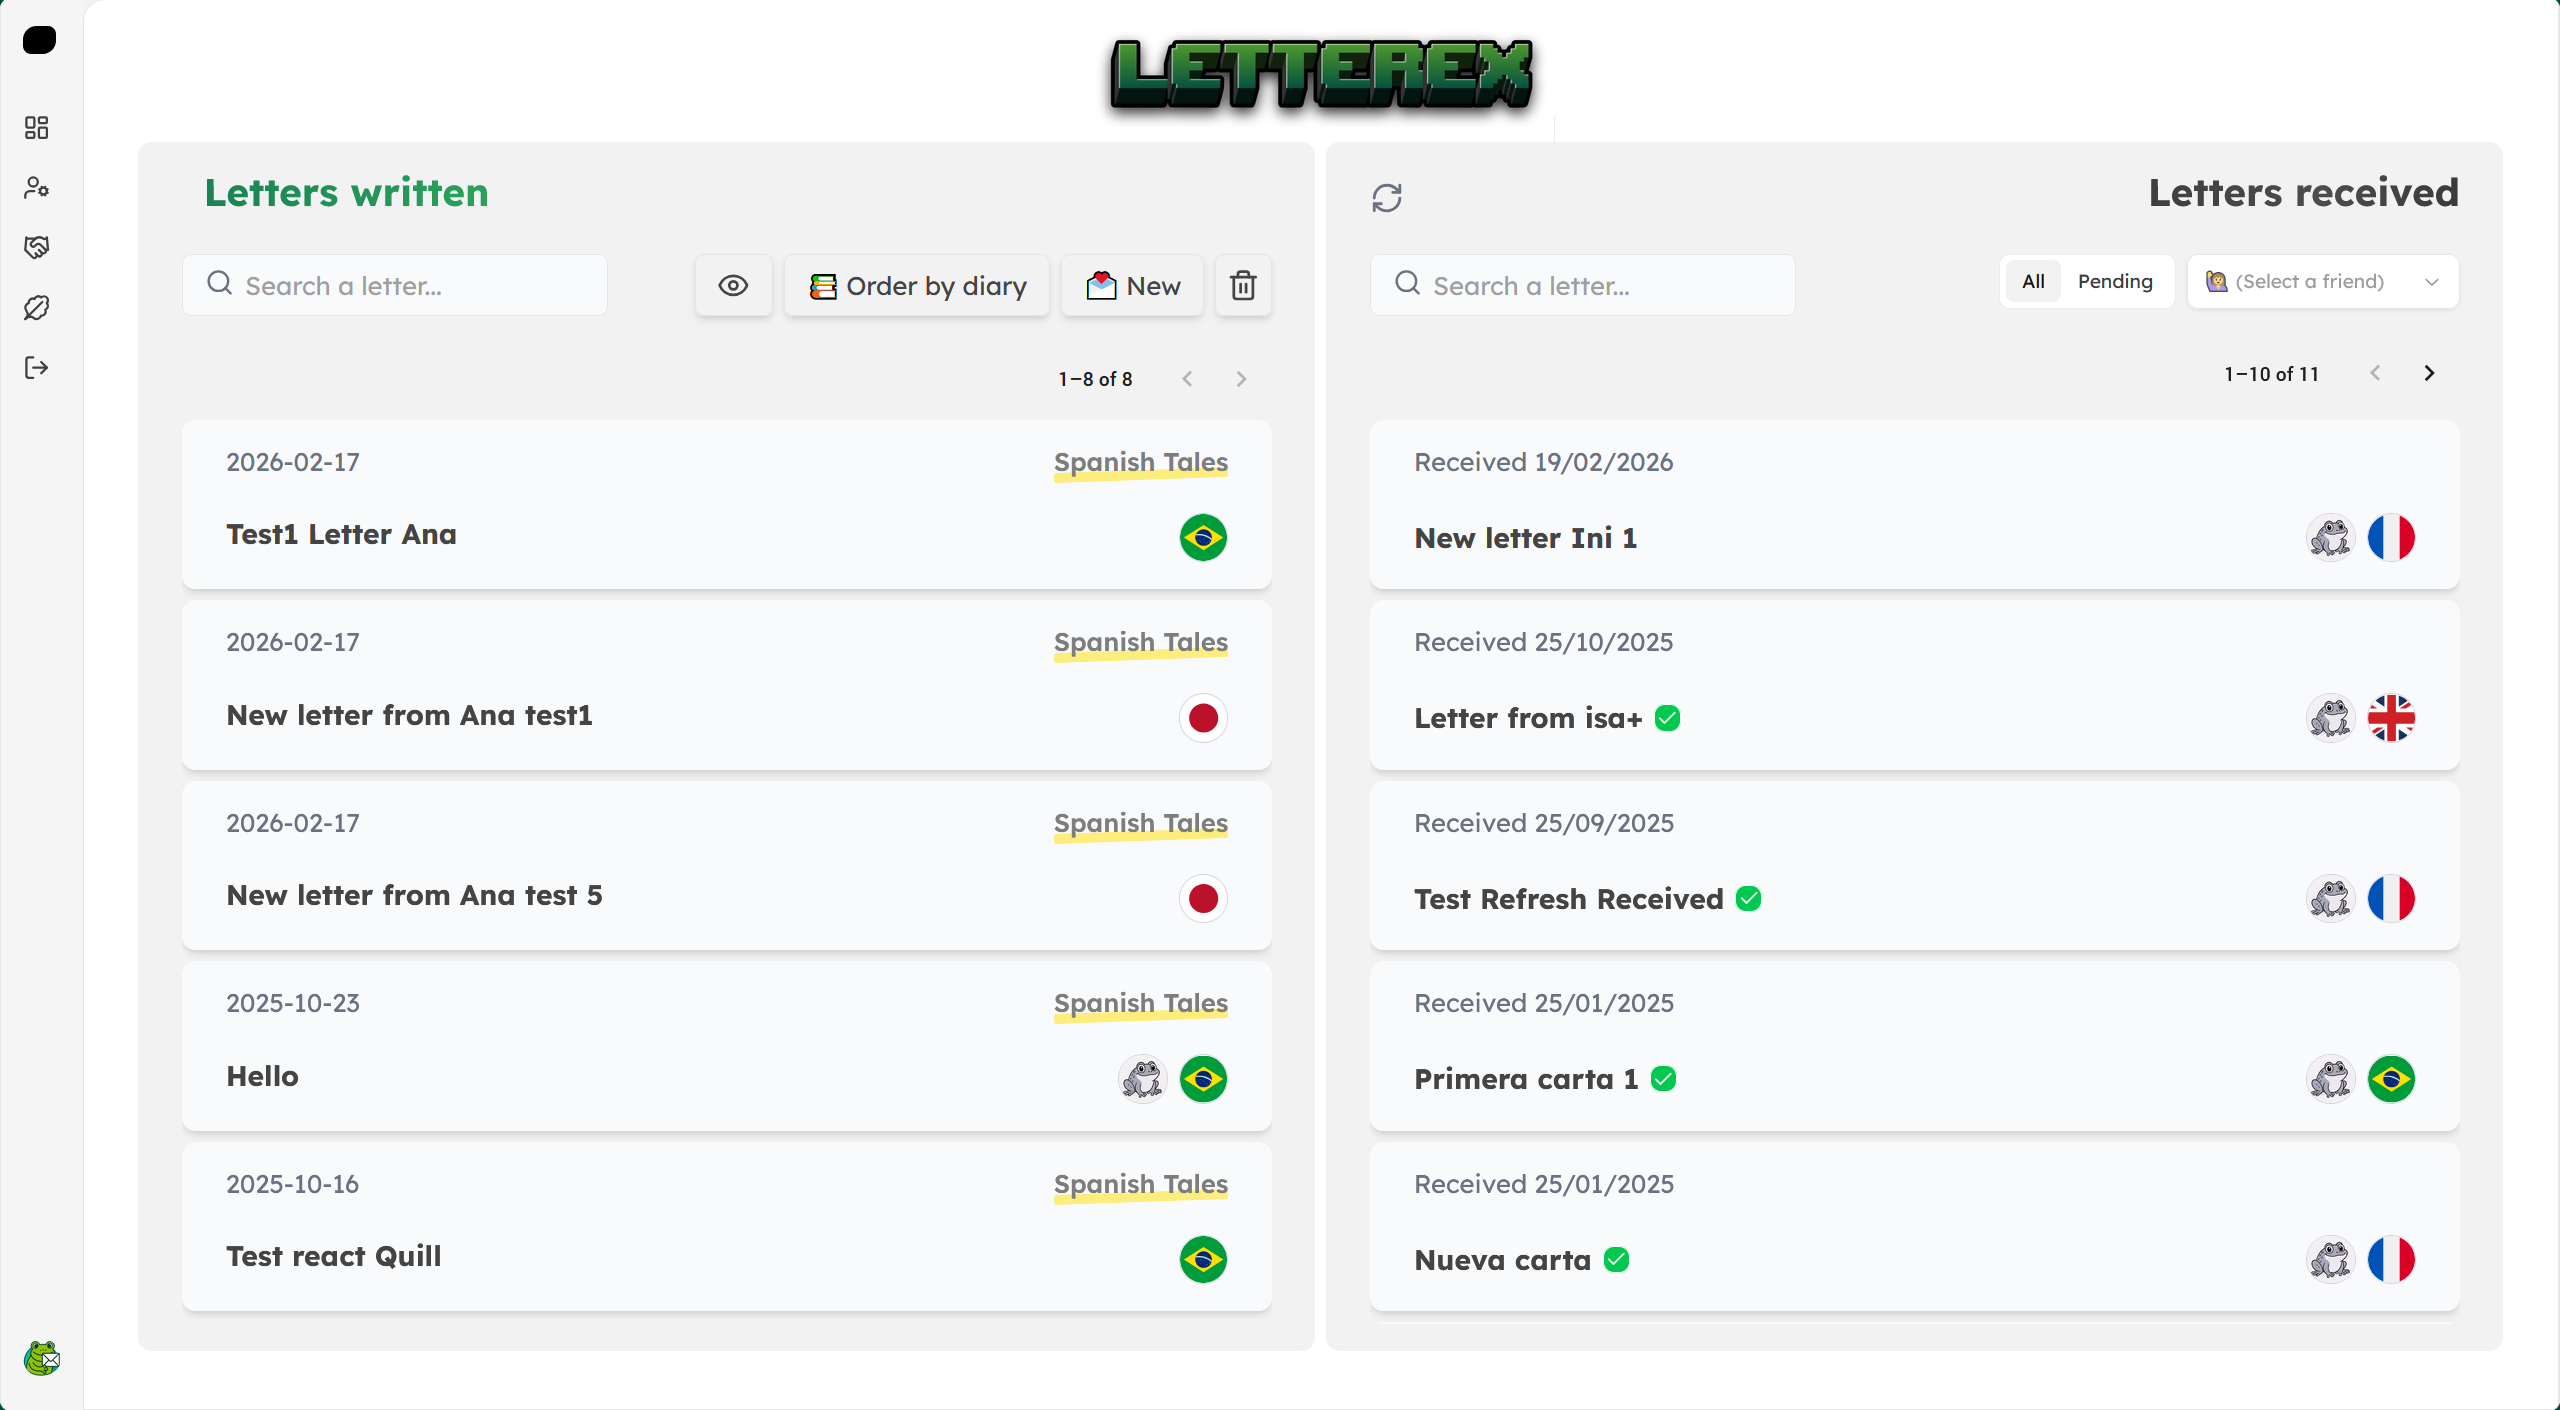
\includegraphics[width=\textwidth]{imagenes/ui/homepage.png}
    \caption{Página principal}
    \label{fig:homepage}
\end{figure}

El dashboard principal (\texttt{/homepage}) es la página central de la aplicación después del inicio de sesión. Está estructurado en dos secciones principales:

\begin{enumerate}
    \item \textbf{Letters Written}: Muestra las cartas que el usuario ha escrito, organizadas en tarjetas interactivas con un efecto de desliz que revela información adicional al interactuar, y paginadas en tandas de 5 elementos. Permite filtrar por una búsqueda, ordenar las cartas por diarios, y eliminar una o varias cartas de la lista. Clicando en la tarjeta de una carta se accede a la página de visualización o edición de esta, clicando en la tarjeta de usuario corrector que aparece al \textit{hover} (posar el cursor sobre el elemento) se accede a la página de visualización de corrección en caso de haberla, y clicando en el botón \textit{New} de la barra de herramientas se accede a la página para crear una nueva carta.
    \item \textbf{Letters Received}: Presenta las cartas recibidas de usuarios que solicitan una corrección por parte del usuario actual, paginadas de la misma forma que las anteriores. Permite filtrar por una búsqueda, por usuario que envió la carta, y por si esa carta está pendiente de corregir (no fue corregida y enviada de vuelta todavía). Clicando en la tarjeta de una carta recibida, se accede a la página de correción de dicha carta.
\end{enumerate}

\subsubsection{Páginas de Creación y Edición de Cartas}

\begin{figure}[h]
    \centering
    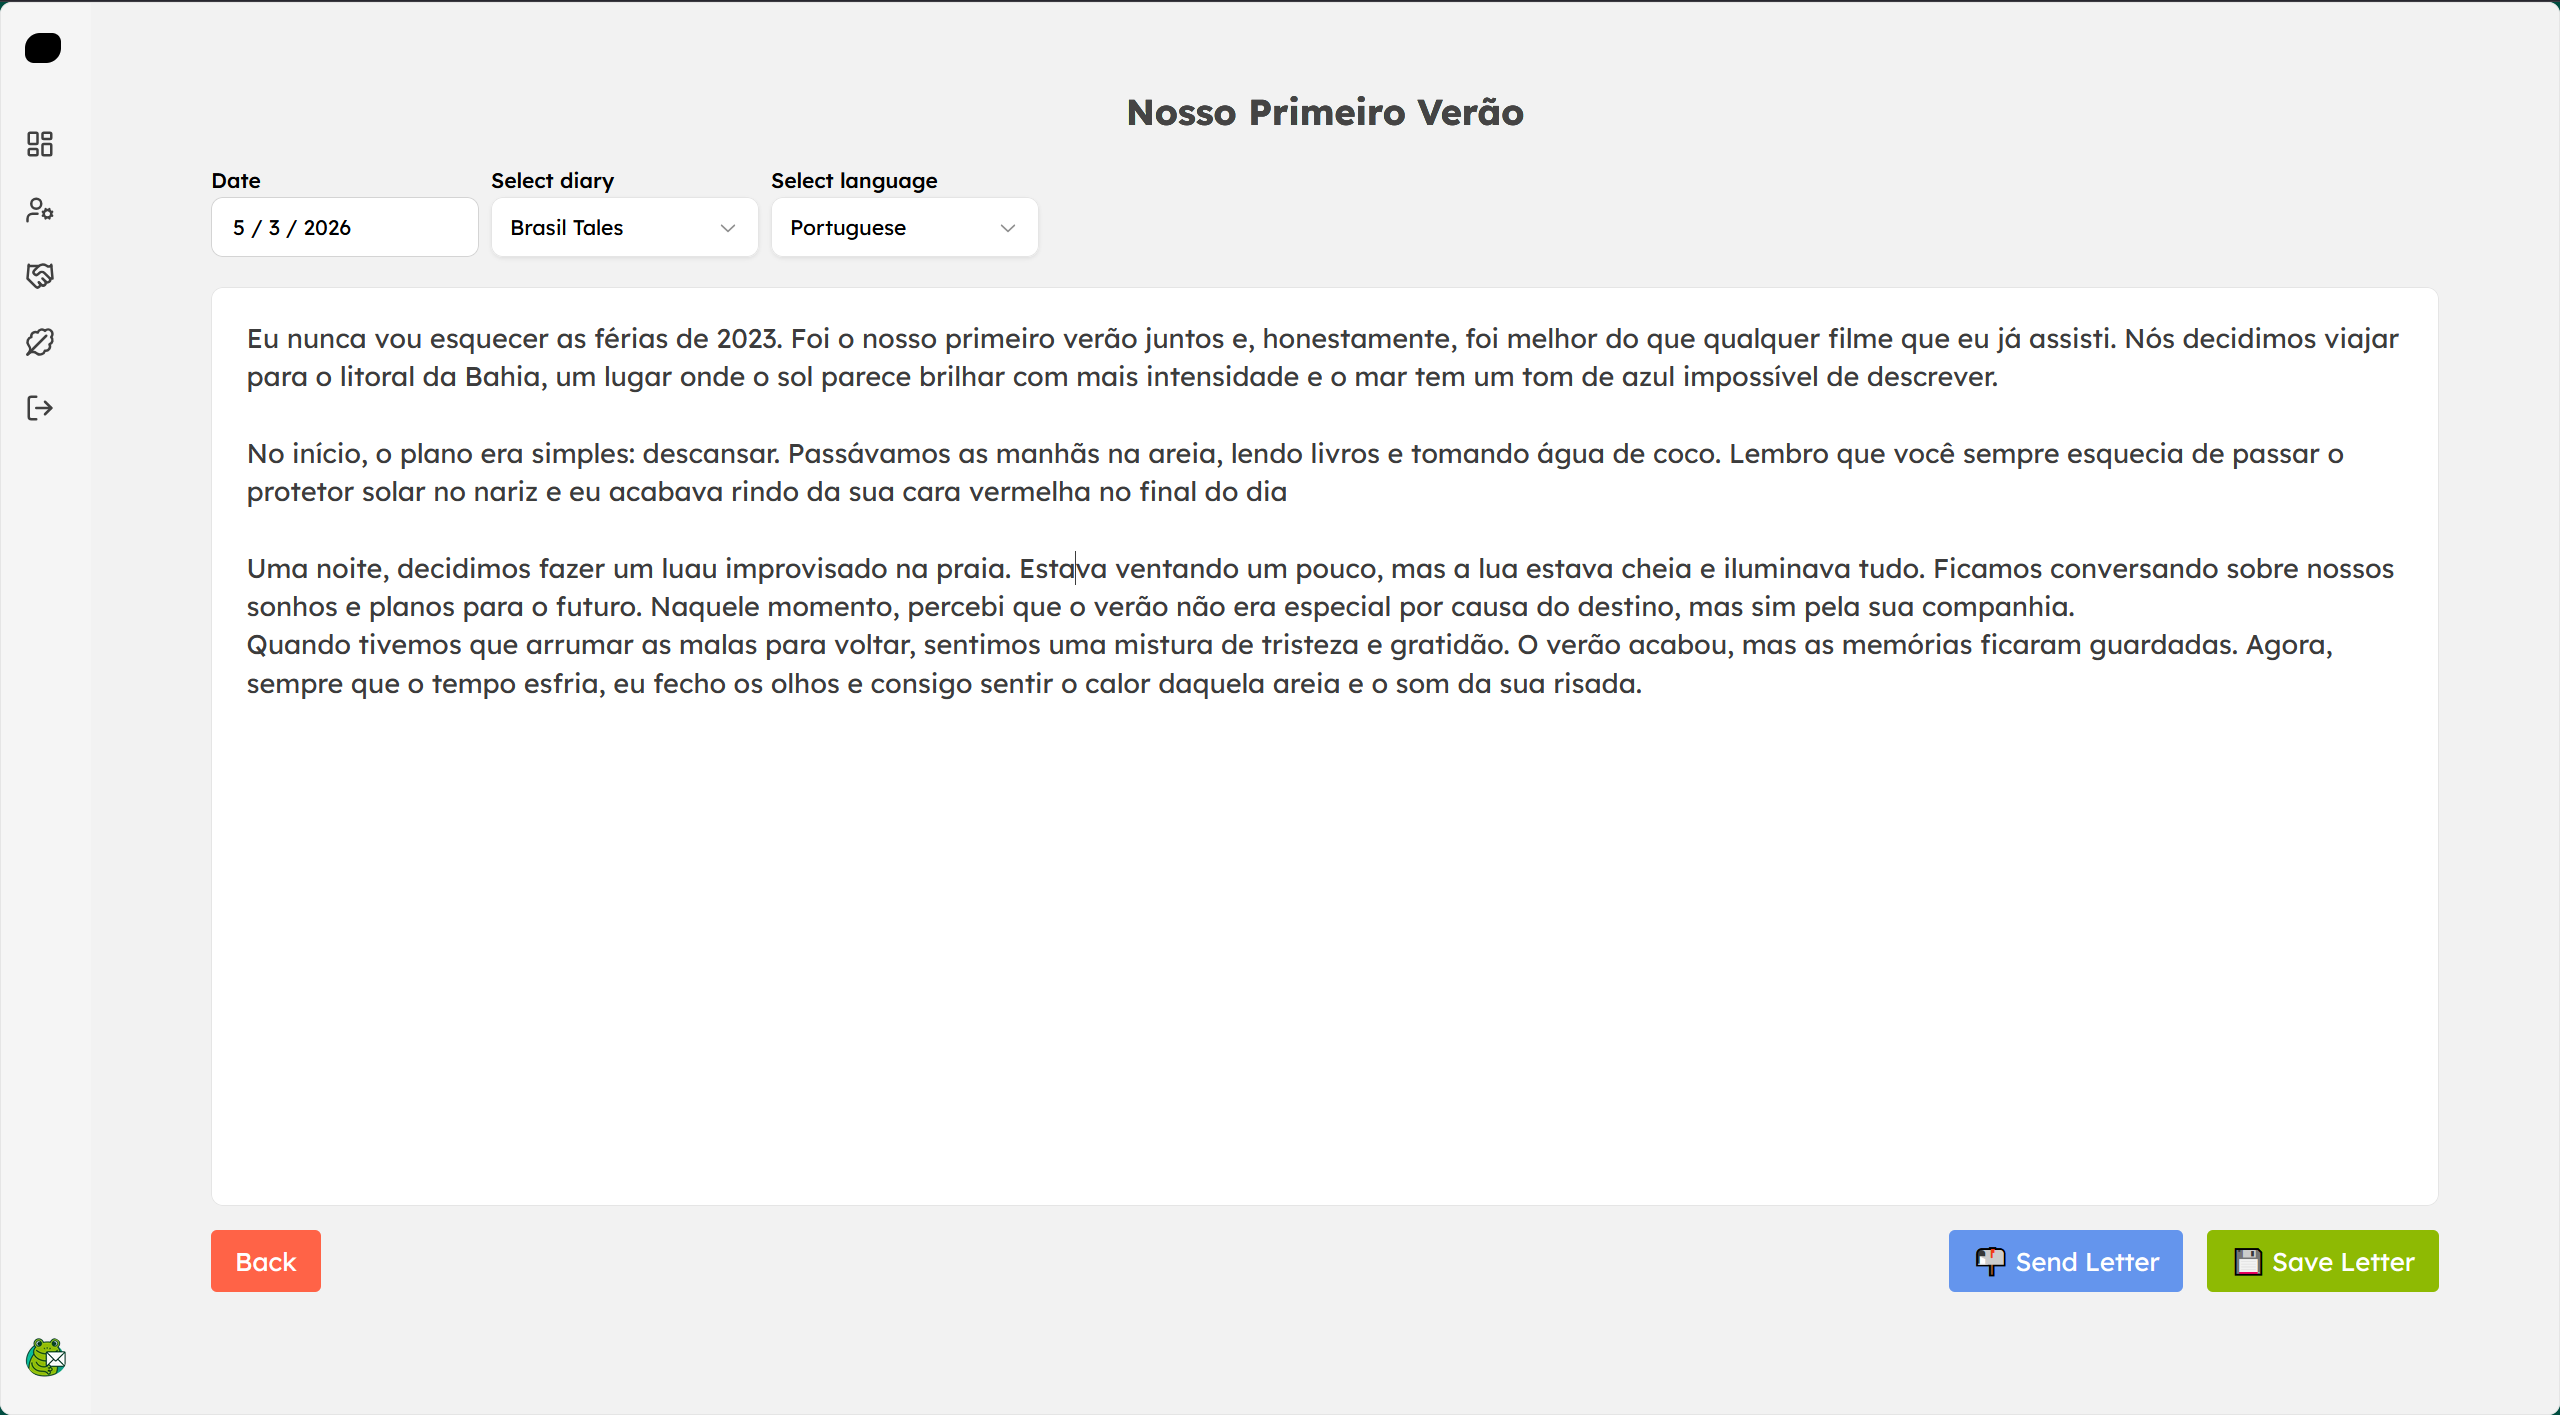
\includegraphics[width=\textwidth]{imagenes/ui/new-letter.png}
    \caption{Página de creación de cartas}
    \label{fig:new-letter}
\end{figure}

La página de creación de cartas (\texttt{/new-letter}) proporciona una interfaz completa para escribir nuevas entradas de diario. El componente implementa validación en tiempo real de los campos requeridos, mostrando mensajes de error específicos cuando el usuario intenta guardar sin completar todos los campos obligatorios. Los elementos principales incluyen campo de título, selectores de fecha, idioma y diario; y un editor de texto enriquecido implementado con React Quill, permite formatear texto con negrita, cursiva, listas, enlaces, etc.\cite{quill_react_playground}

Al guardar la carta, se redirige al usuario a una página muy similar (\texttt{/edit-letter}), lo que permite el guardado de borradores de forma que se pueda seguir editando la carta en otro momento. Esta última página es muy similar a la de Creación de Cartas, salvo que en ella es posible enviar la carta a amigos para que la corrigan.

\subsubsection{Página de Corrección de Cartas}

\begin{figure}[h]
    \centering
    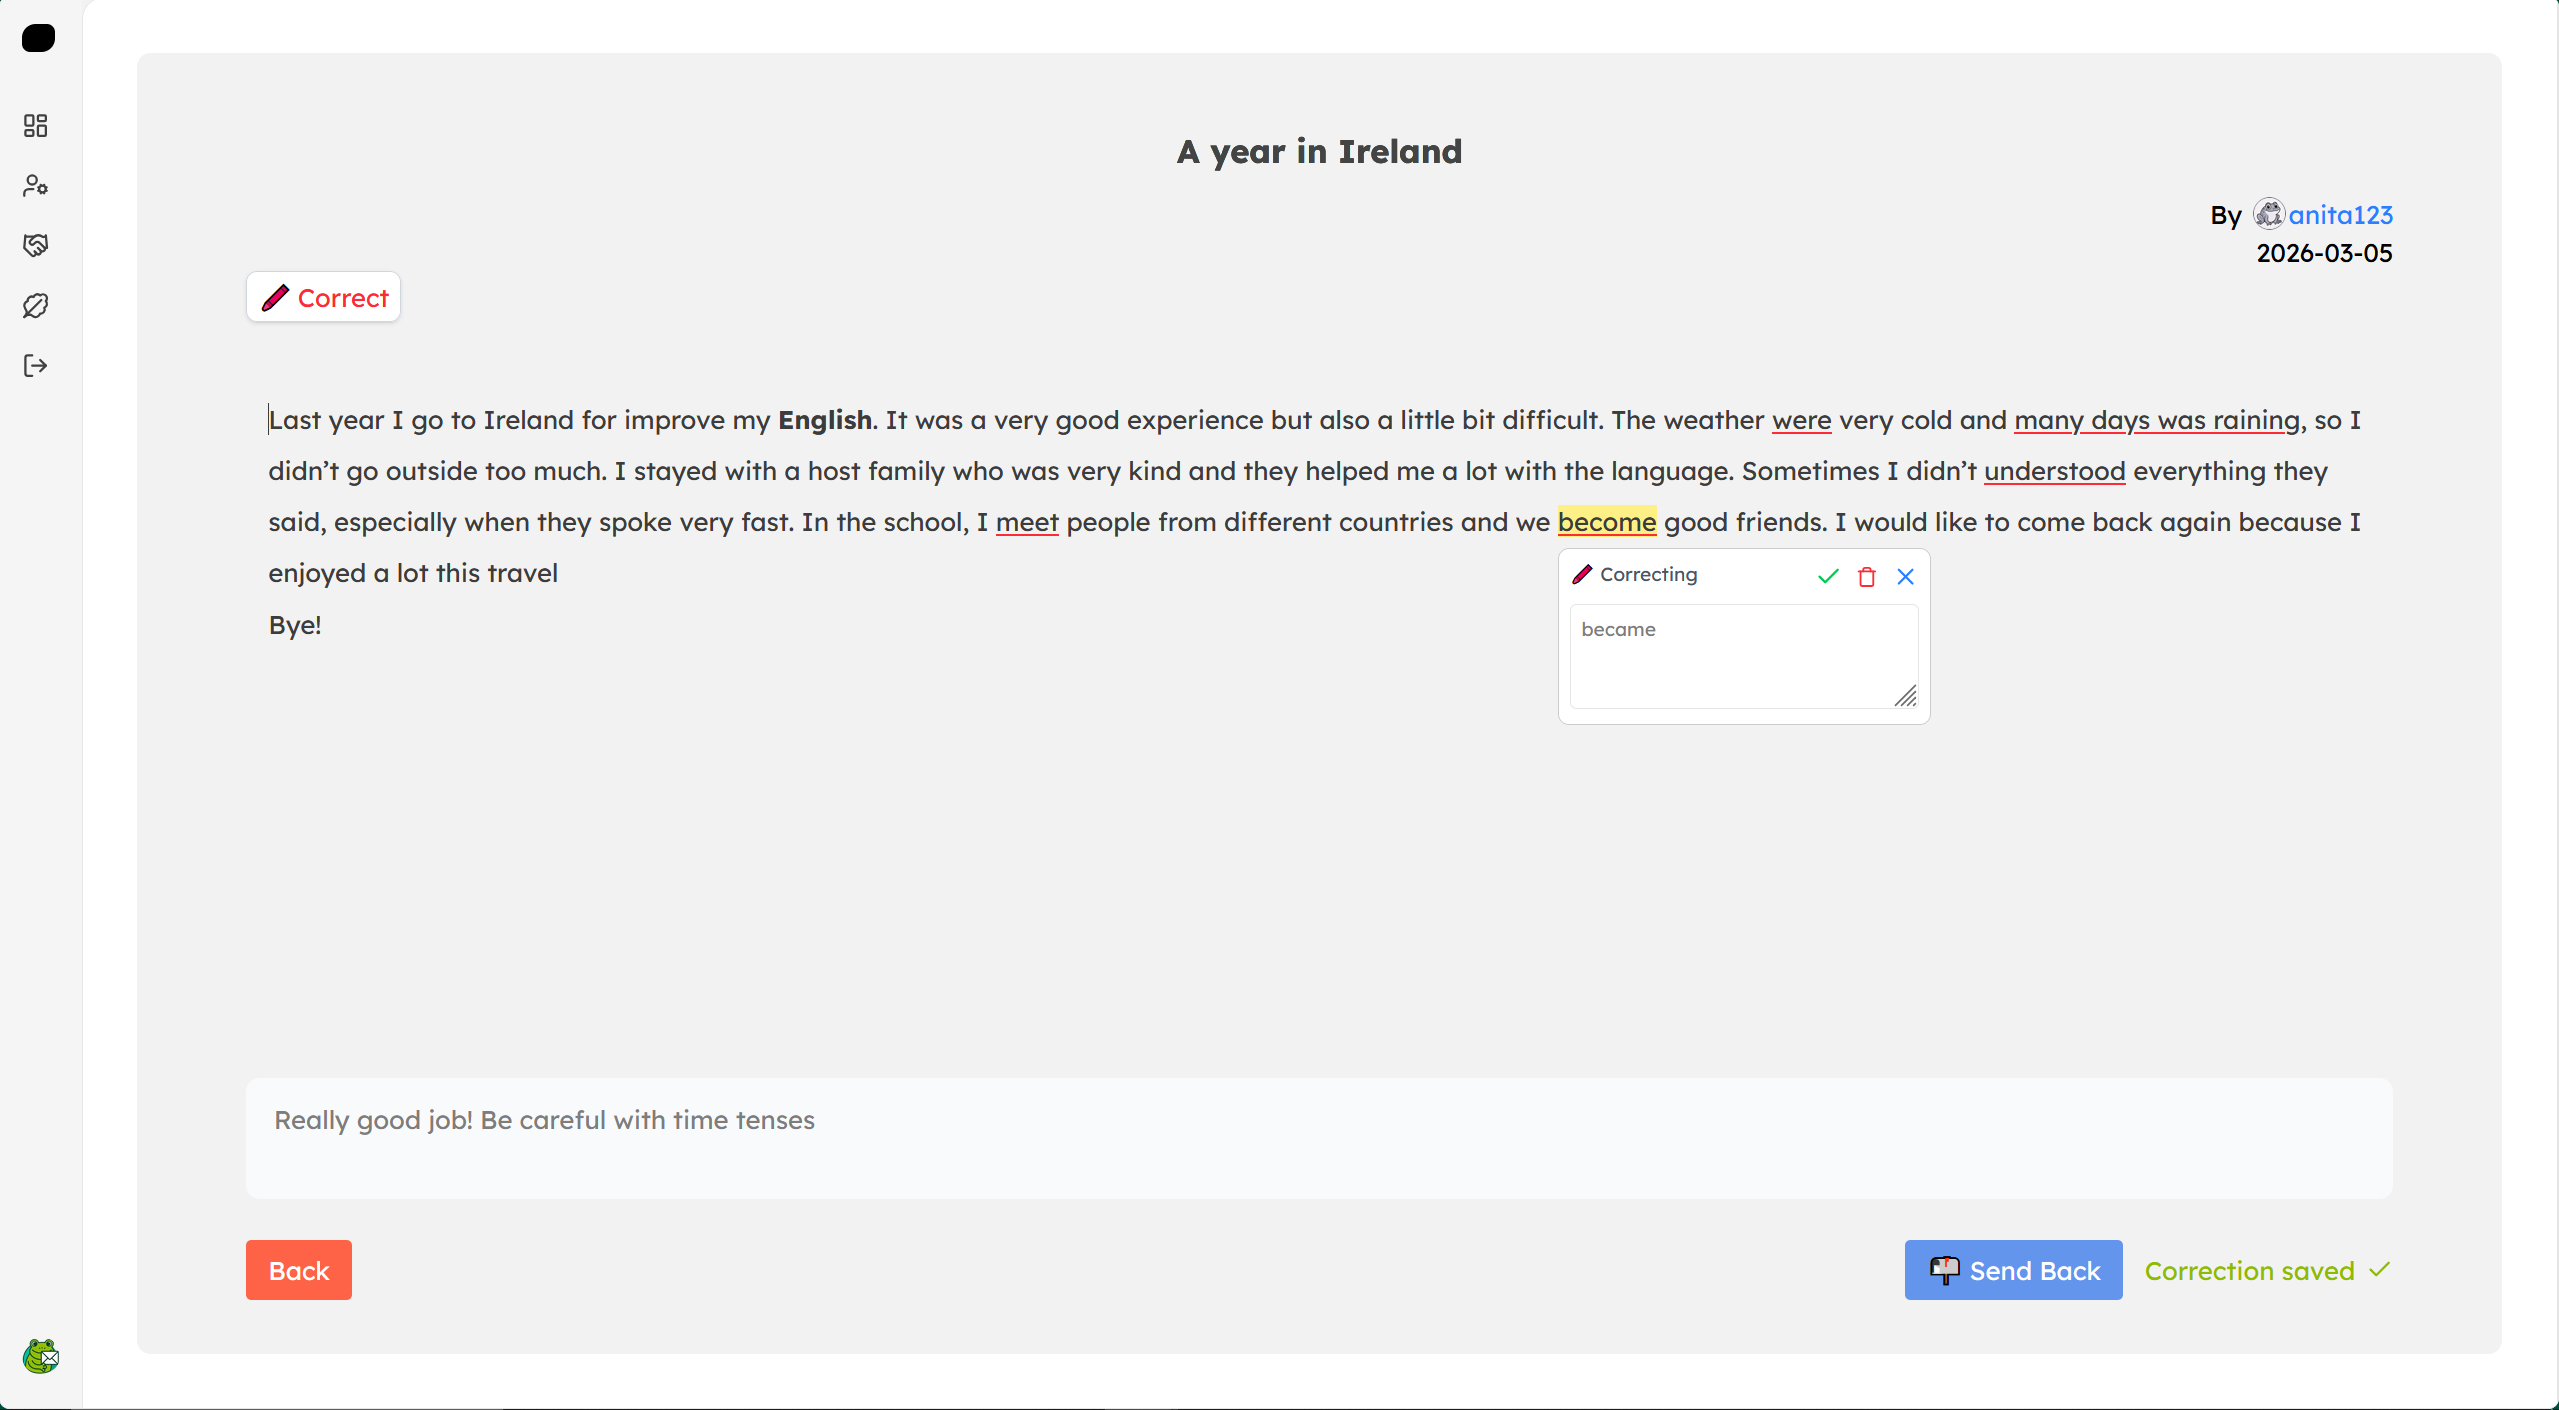
\includegraphics[width=\textwidth]{imagenes/ui/correct-letter2.png}
    \caption{Página de corrección de cartas}
    \label{fig:correct-letter}
\end{figure}

Esta página (\texttt{/correct-letter}) permite a los usuarios corregir las cartas escritas por otros en idiomas que dominan.

Para añadir correcciones, el usuario debe seleccionar fragmentos específicos del texto original que considere que contienen errores o se puede matizar. El texto seleccionado se resalta visualmente, y se abre un panel de escritura para asociarlo con una corrección sugerida o un comentario explicativo. Además de las correcciones específicas, el corrector puede dejar un comentario general sobre la carta al final.

El componente \texttt{TextCorrections} renderiza de forma dinámica el texto con las correcciones aplicadas. El proceso incluye:

\begin{enumerate}
    \item Parseo del texto original: Se divide el texto en fragmentos según las posiciones de corrección.
    \item Detección de solapamientos: Antes de añadir una nueva corrección, se verifica que no se solape con correcciones existentes mediante comparación de índices.
    \item Renderizado diferenciado: Cada fragmento se renderiza con estilos diferentes según sea texto sin corregir o texto corregido. Concretamente, el texto corregido va marcado en amarillo al hover y subrayado en rojo.
    \item Interactividad: Los fragmentos corregidos son interactivos. Al clicar en ellos o pasar el cursor, se abre un panel donde se pueden añadir o editar las correcciones.
\end{enumerate}

Para hacer esto posible, esta es la estructura de datos que se asocia a una corrección:

\begin{center}
\begin{minipage}{0.36\textwidth}
\begin{verbatim}
interface Correction {
    id: string;
    startIndex: number;
    endIndex: number;
    originalText: string;
    correctedText: string;
}
\end{verbatim}
\end{minipage}
\end{center}

\subsubsection{Página de Visualización de Correcciones Recibidas}

\begin{figure}[h]
    \centering
    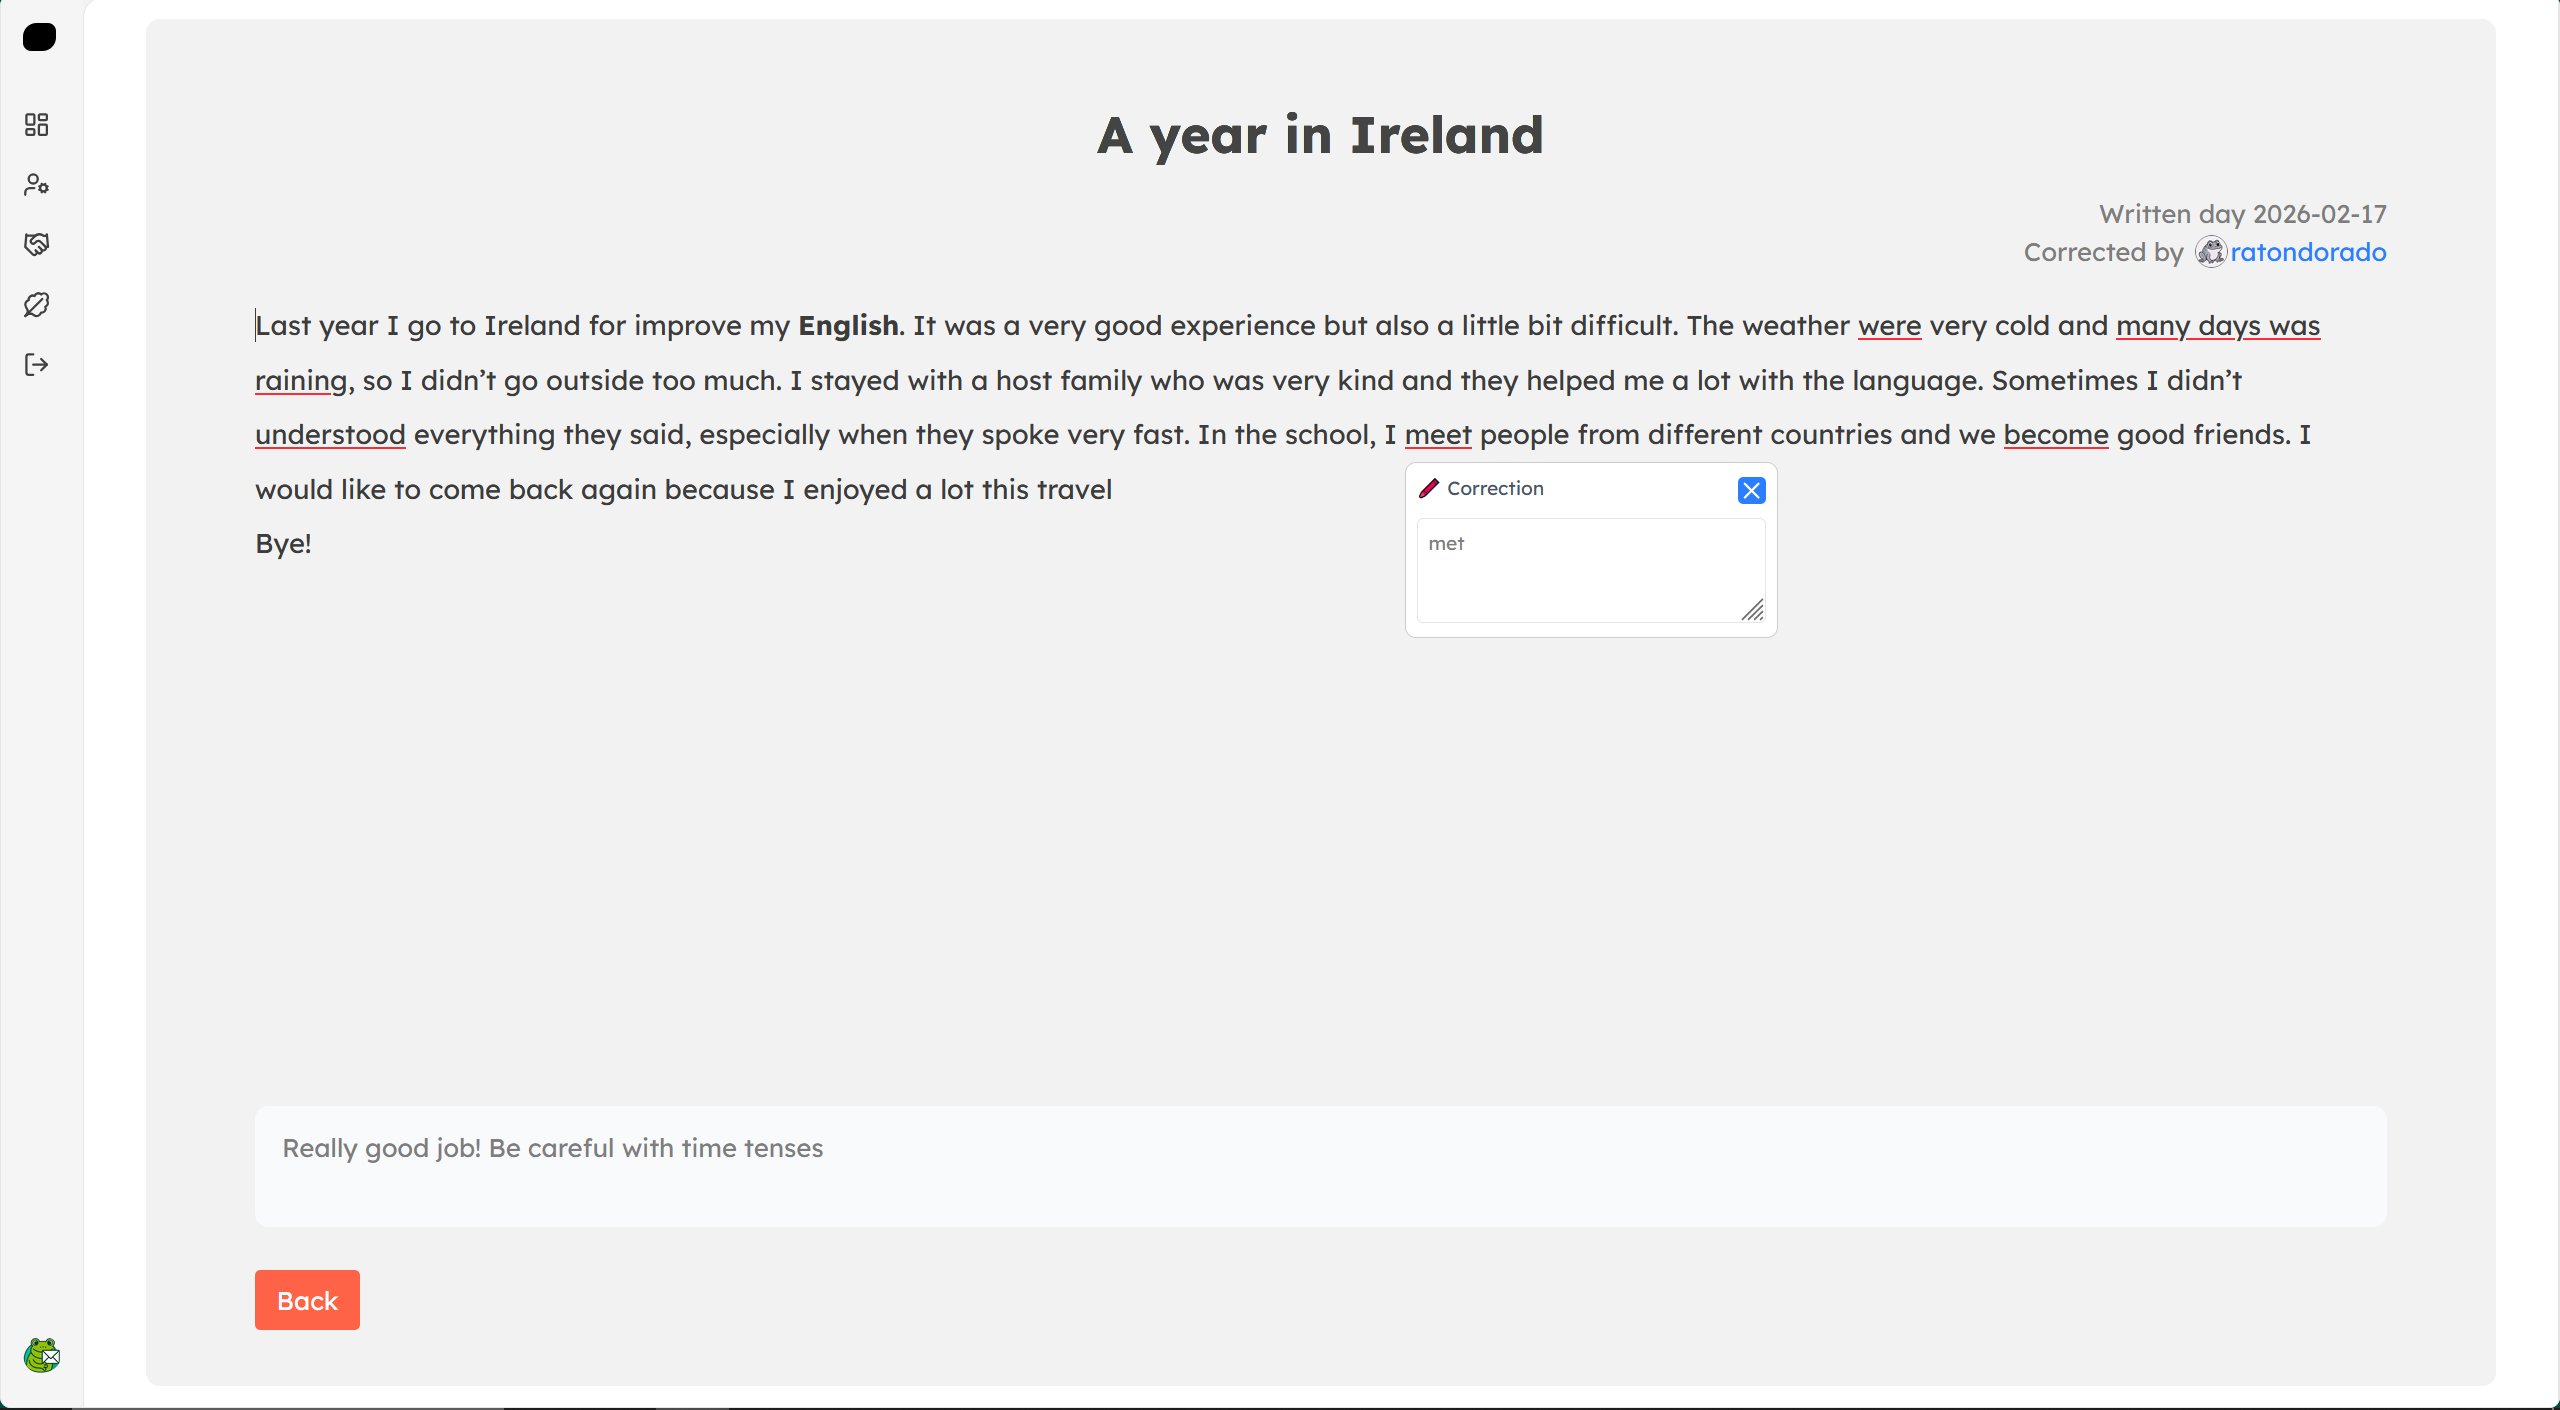
\includegraphics[width=\textwidth]{imagenes/ui/view-correction.png}
    \caption{Página de visualización de corrección recibida}
    \label{fig:view-correction}
\end{figure}

La página de visualización (\texttt{/view-correction}) de correcciones presenta al usuario remitente las correcciones recibidas en sus cartas. Esta interfaz permite al usuario aprender de sus errores de forma efectiva, clara y visualmente agradable. La interfaz es similar a la de Corrección de Cartas, pero sin permitir editar o enviar la corrección.

Se muestra el texto original con las secciones corregidas resaltadas en color diferenciado. Al hacer click o hover sobre una sección corregida, se muestra un panel con la corrección sugerida. Se muestran también los comentarios generales del corrector sobre la carta, y la información del corrector (nombre e imagen de perfil), que actúa como enlace a su página de perfil.

\subsubsection{Página de Amigos}

\begin{figure}[h]
    \centering
    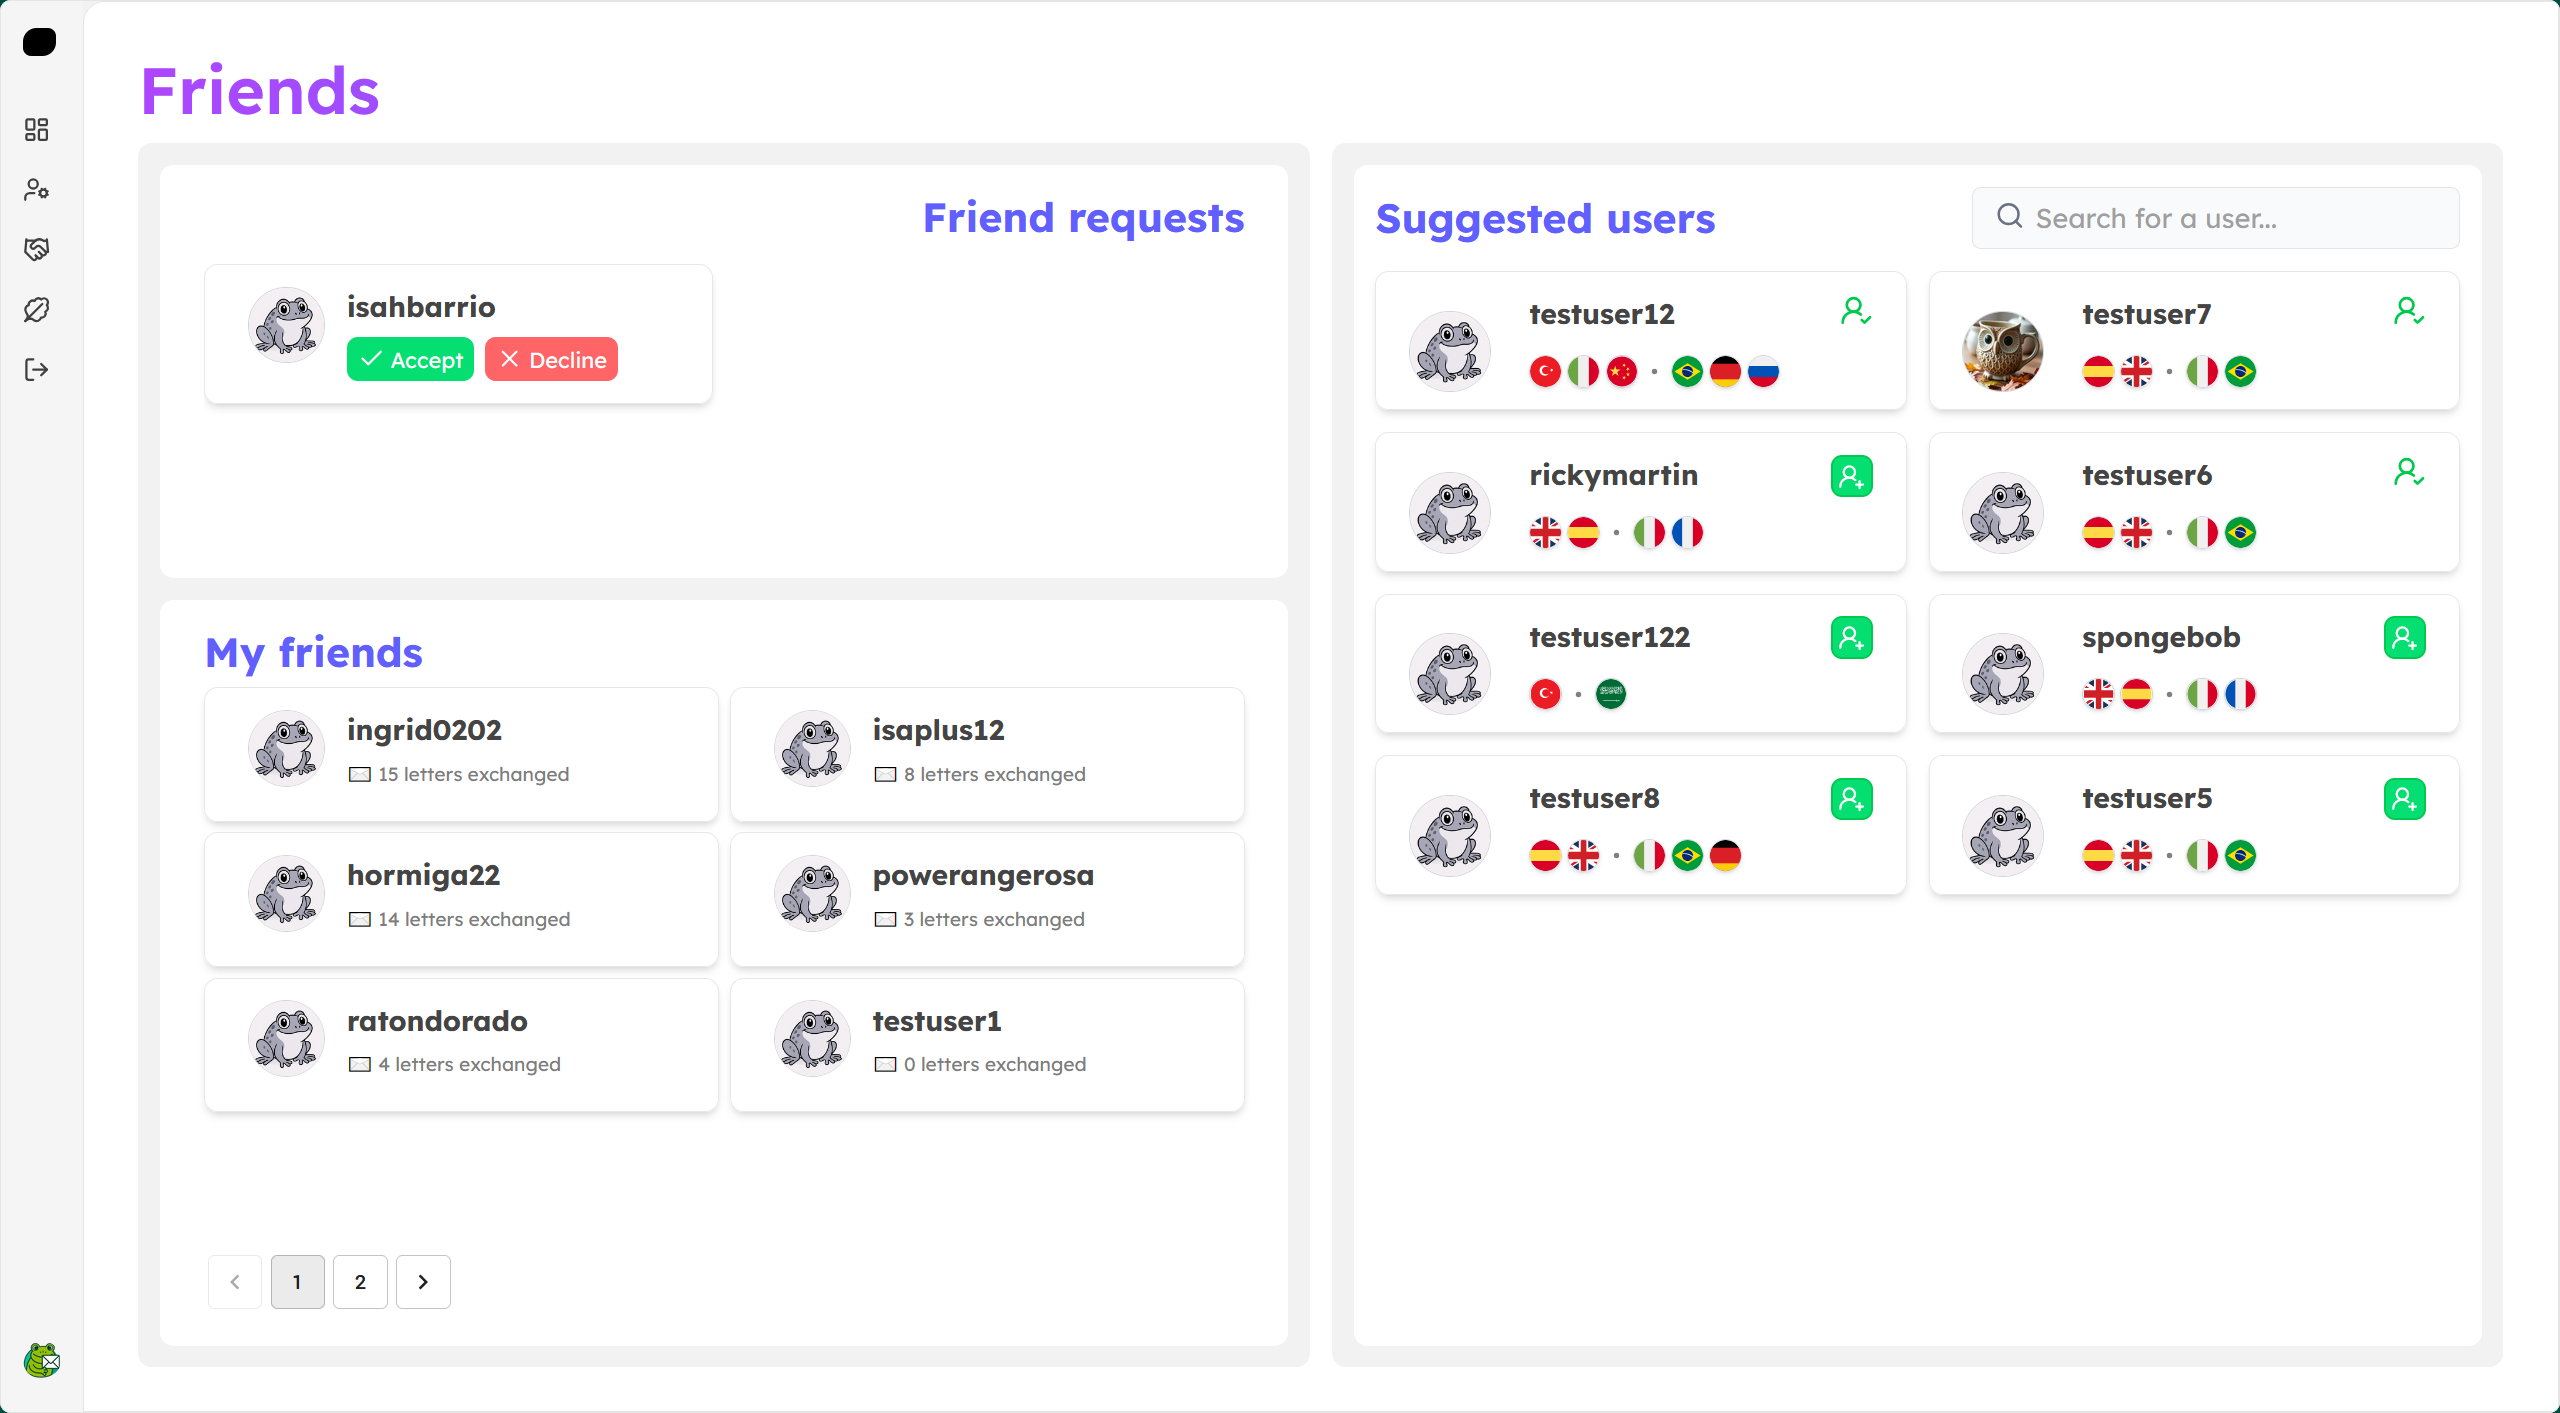
\includegraphics[width=\textwidth]{imagenes/ui/friends-page.png}
    \caption{Página de amigos}
    \label{fig:friends}
\end{figure}

En la página de amigos (\texttt{/friends}), el usuario puede gestionar las relaciones sociales dentro de la aplicación. Se divide en tres secciones:

\begin{enumerate}
    \item \textbf{Solicitudes de amistad}: Muestra las solicitudes pendientes recibidas, con opciones para aceptar o rechazar.
    \item \textbf{Lista de amigos}: Presenta las amistades establecidas con su avatar, nombre y estadísticas como el número de cartas intercambiadas.
    \item \textbf{Usuarios sugeridos}: Muestra usuarios recomendados basándose en idiomas en común, además de un buscador por nombre de usuario para poder encontrar un usuario en concreto que se desee agregar.
\end{enumerate}

La página implementa paginación para todas estas listas de usuarios y solicitudes. También, al clicar cualquiera de las tarjetas de usuario, se accede a la página de perfil de este.

\subsubsection{Página de Perfil de Usuario}

\begin{figure}[H]
    \centering
    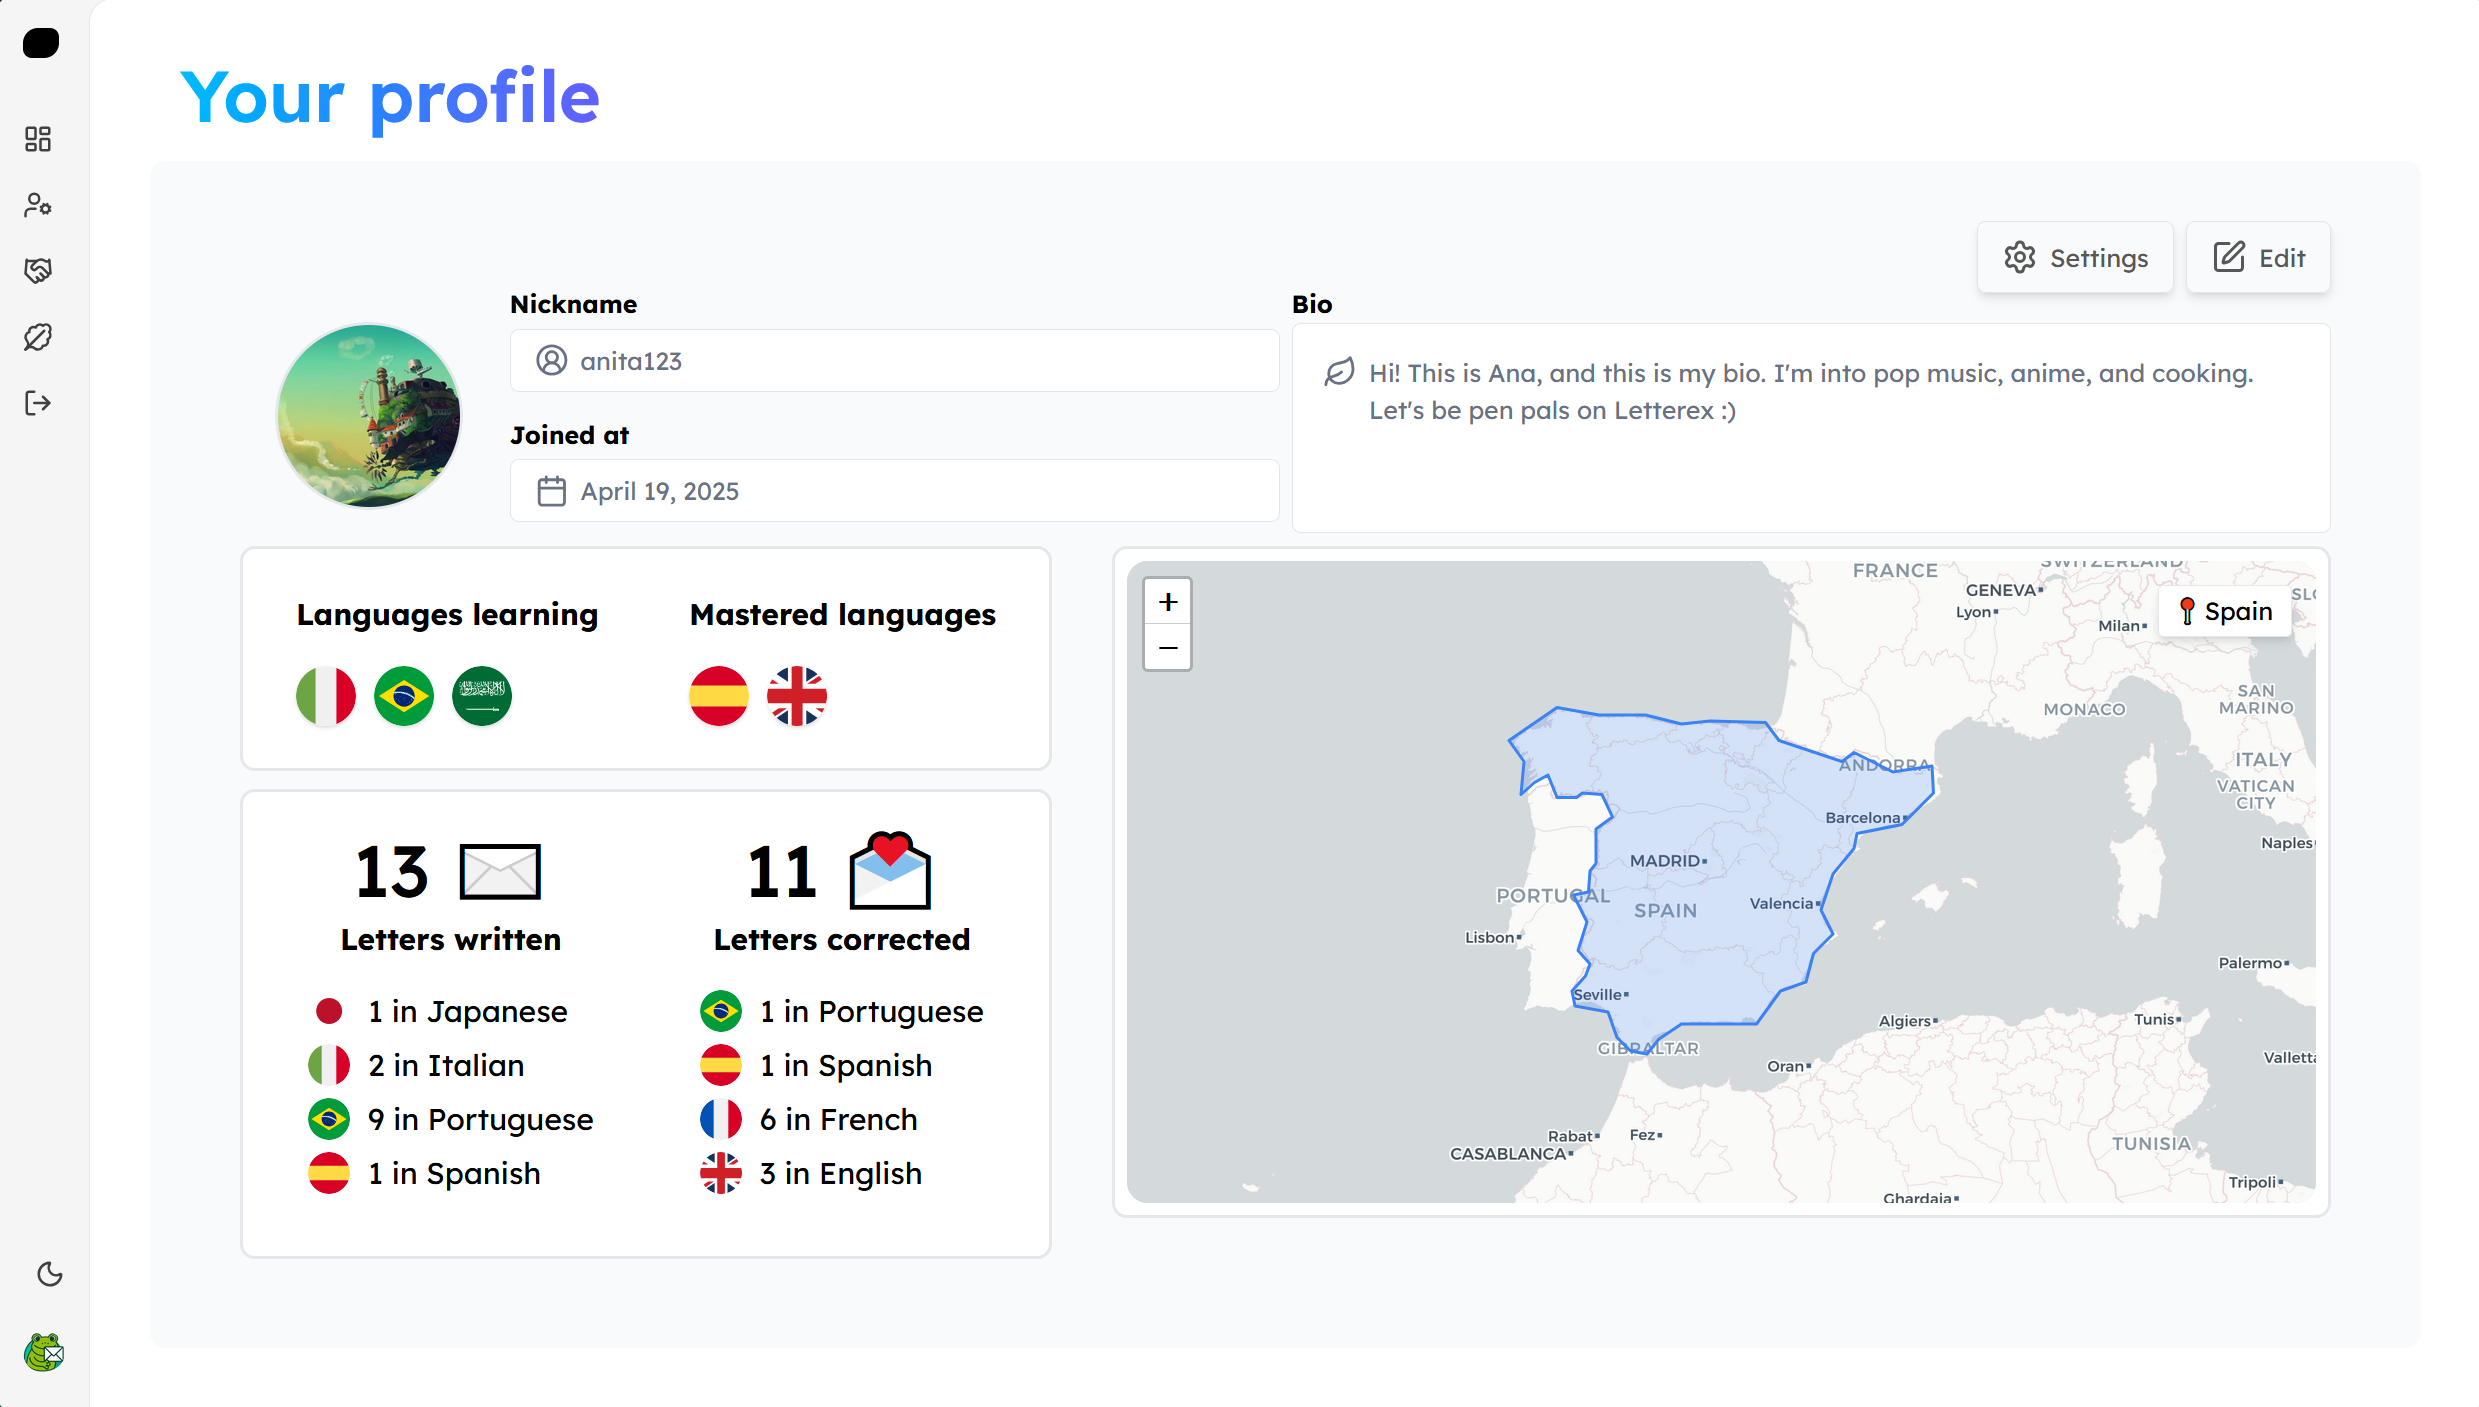
\includegraphics[width=\textwidth]{imagenes/ui/my-profile.png}
    \caption{Página de perfil de usuario}
    \label{fig:profile}
\end{figure}

La página de perfil muestra información detallada sobre un usuario. Se utiliza la misma página para el perfil propio y para el de otros usuarios. La página incluye:

\begin{itemize}[label={-}]
    \item Foto de perfil, nombre y biografía.
    \item Idiomas nativos y lenguas que está aprendiendo.
    \item Estadísticas de cartas escritas y corregidas en cada idioma.
    \item Ubicación geográfica visualizada en un mapa interactivo de React Leaflet.
    \item Para el perfil de usuario ajeno, un botón para dar la opción de eliminar de la lista de amigos en caso de tener a ese usuario agregado.
    \item Para el perfil de usuario autenticado (mi perfil), opciones de edición de la información del perfil y de configuración (cambiar contraseña o eliminar la cuenta).
\end{itemize}

\subsection{Técnicas de Optimización}

Finalmente, al igual que en el backend, en el frontend se han implementado varias técnicas de optimización. Estas técnicas se han aplicado de forma complementaria y selectiva, con el objetivo de mejorar el rendimiento de la aplicación y la experiencia de usuario en distintos niveles: carga de recursos, fluidez de la navegación, renderizado de componentes y comunicación con el backend.

\begin{enumerate}
    \item \textbf{Importaciones Dinámicas}: Componentes pesados como el mapa de la página de perfil se cargan dinámicamente solo cuando son necesarios. Esto es posible gracias a la función \texttt{dynamic} de Next.js, diseñada para optimizar el rendimiento mediante la técnica de carga diferida (\textit{Lazy Loading}) de los componentes, que asegura que el navegador descargue el código de estos componentes no al inicio sino en el momento en que los necesite. Mientras se carga, aparece un mensaje para informar al usuario del estado de carga.
    \begin{verbatim}
        const ImageUploader = dynamic(
            () => import("@/components/imageUploader"),
            { loading: () => <div>Loading...</div> }
        );
    \end{verbatim}

    \item \textbf{Memoización}: En la app se usan las funciones de React \texttt{useCallback} y \texttt{useMemo} para evitar recrear funciones y recalcular datos en cada renderizado.

    \item \textbf{Paginación}: Las listas de registros (cartas, correcciones, amigos) incluyen paginación para reducir la cantidad de datos cargados y renderizados simultáneamente. Se cargarán más elementos del servidor solo cuando el usuario lo solicite pasando de página en la lista.

    \item \textbf{Debouncing}: En campos de búsqueda y filtrado, se implementa debouncing para reducir el número de llamadas a la API, como se ha descrito en la sección anterior de arquitectura del backend.

    \item \textbf{Lazy Loading de imágenes}: Las imágenes de perfil se cargan de forma diferida para mejorar el tiempo de carga inicial.

    \item \textbf{Pantallas esqueleto}: Para mejorar la experiencia del usuario durante la carga de datos, se han utilizado pantallas esqueleto (\textit{skeleton screens}). Se genera una estructura visual gris translúcida que replica la de la página real (títulos, bloques de contenido, botones...) mientras se cargan los datos del servidor. Esto reduce la sensación de espera porque el usuario ya ve dónde aparecerá cada elemento. Una vez que los datos llegan, el esqueleto se reemplaza con el contenido definitivo.

    \begin{figure}[H]
        \centering
        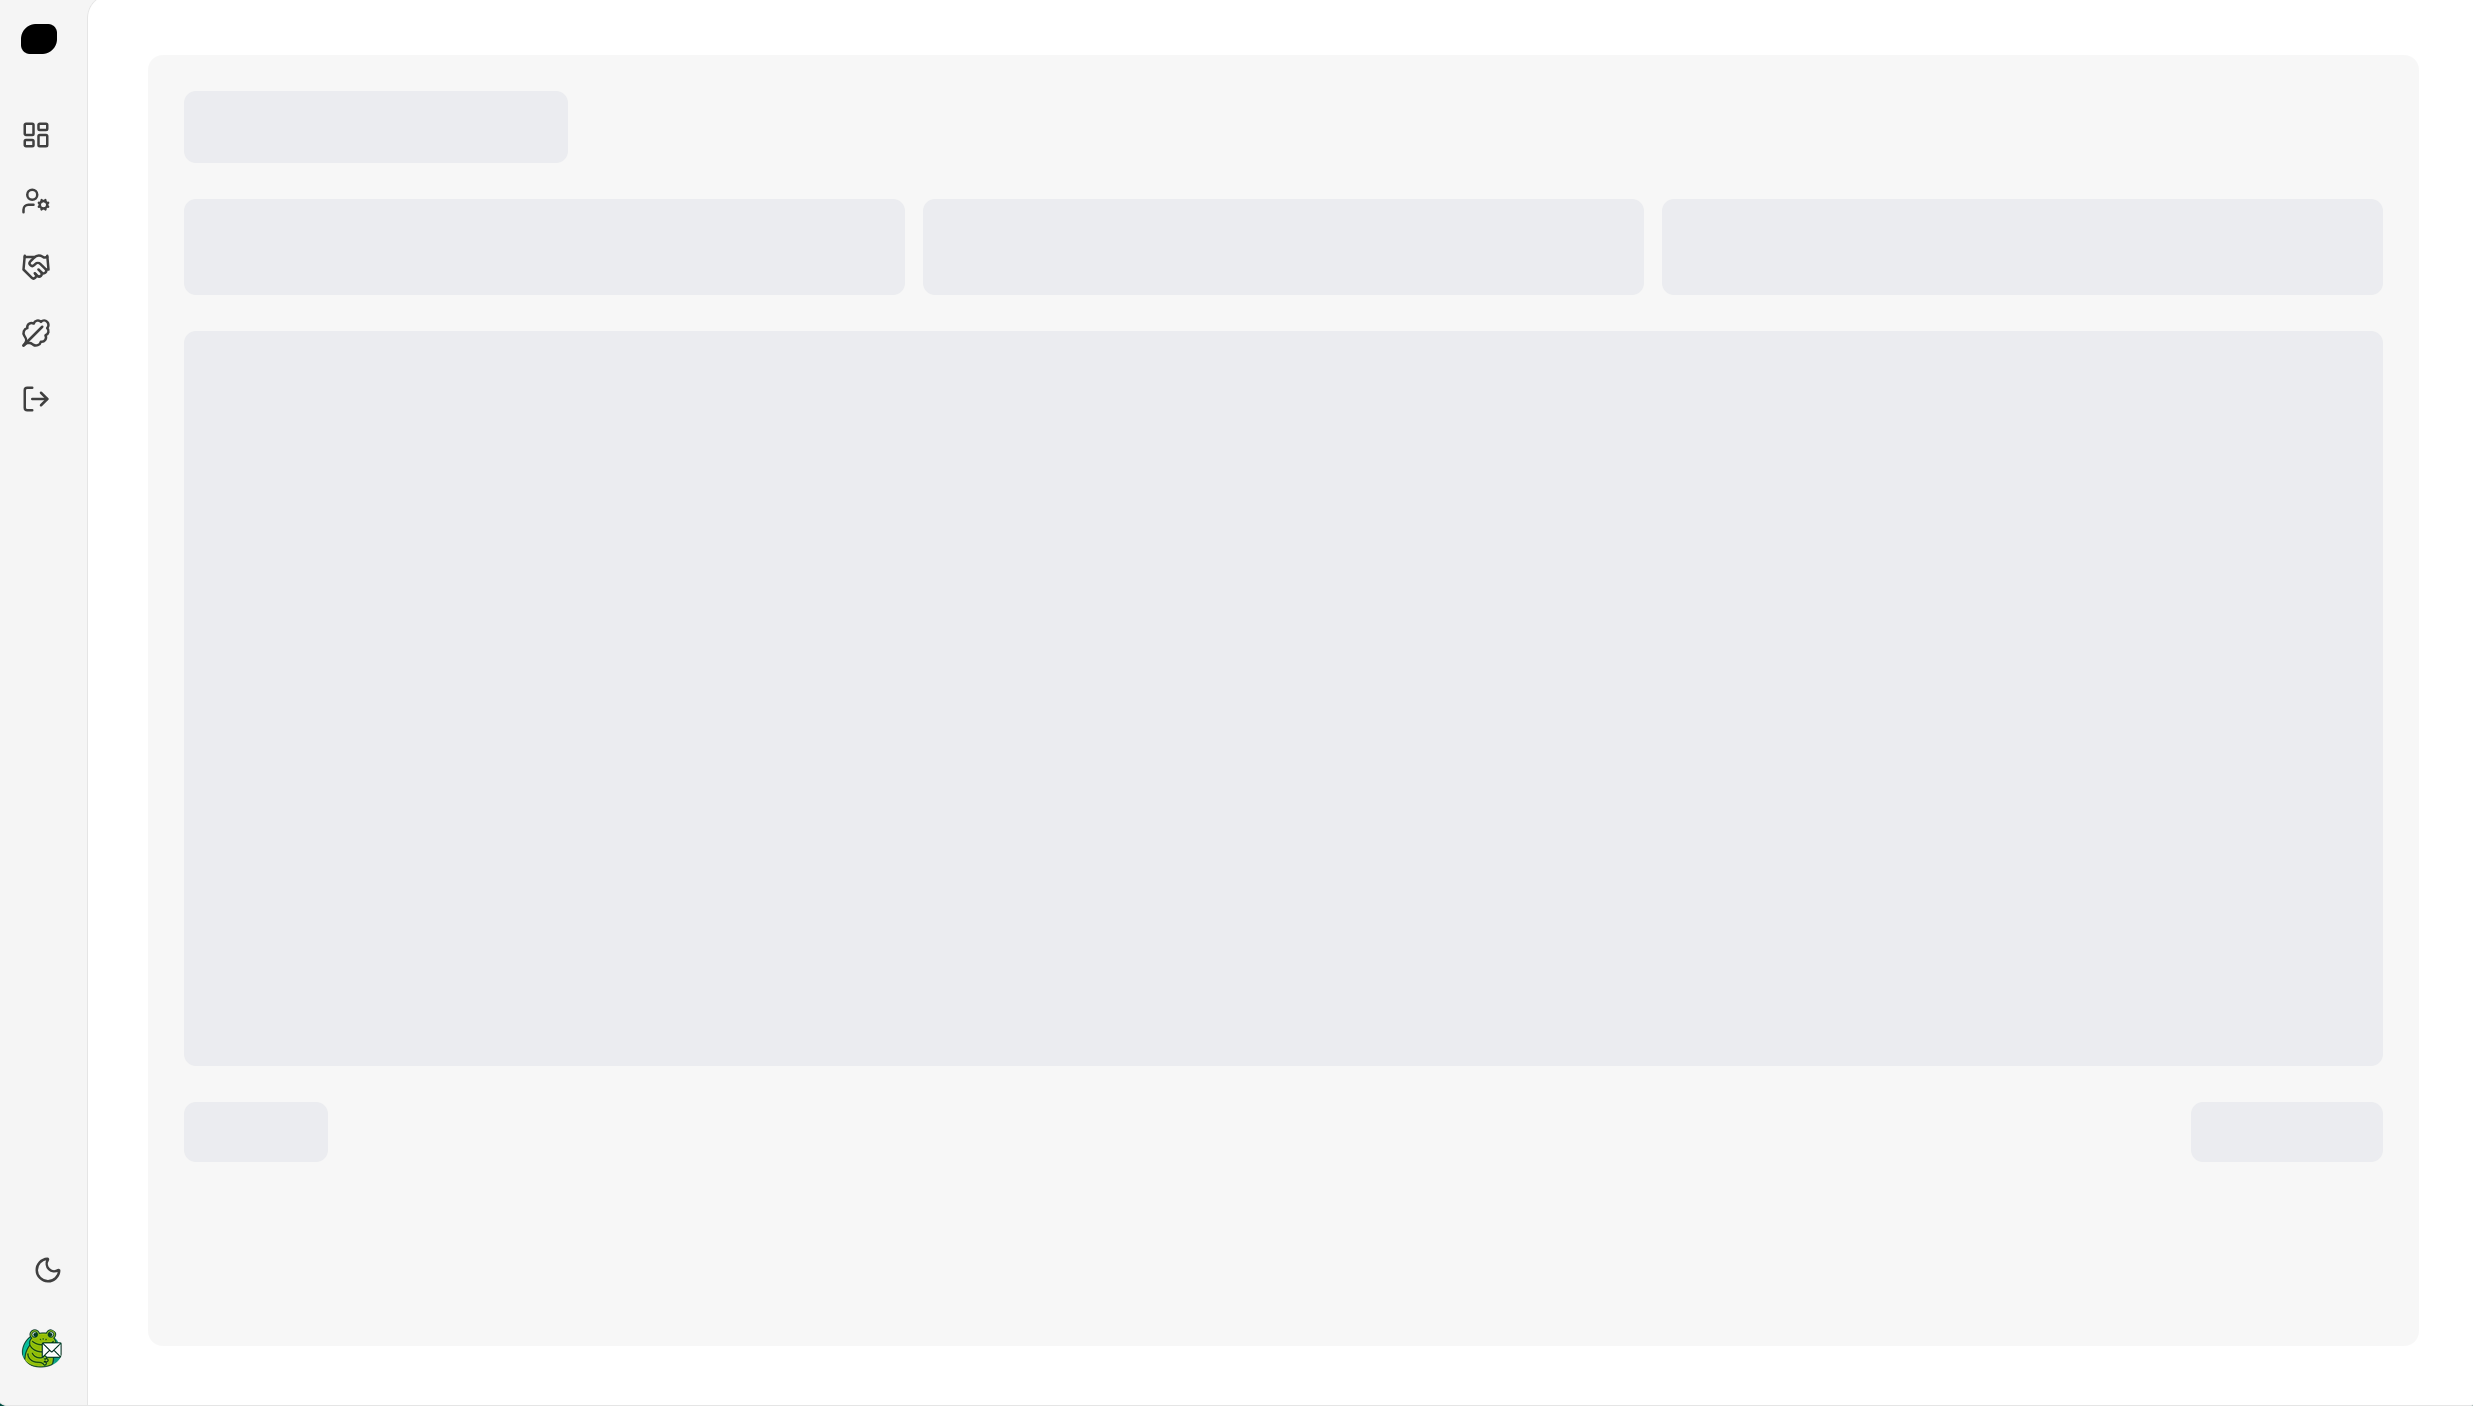
\includegraphics[width=\textwidth]{imagenes/ui/skeleton.png}
        \caption{Ejemplo de Pantalla Esqueleto}
        \label{fig:skeleton}
    \end{figure}
\end{enumerate}

